 % The main file for CAMP reports
 % Don't put any content in here. 
 % Don't even include content files by using \input or \inlcude. 
 % Put your content to TEXT.TEX or include it there using \input.
 % Uses:
 %		SETTINGS.TEX	contains the settings for this document
 %		COMMANDS.TEX	contains commands which can be used while writing
 %		INFO.TEX			contains the author, title and so on for the cover
 %		COVER.TEX			formats the front cover of the document
 %		ABSTRACT.TEX	contains the abstract to be included (if needed)
 %		TEXT.TEX			contains the actual content of the document
 %		BIB.BIB				containt the BibTeX entries for the document
 
 
%% Draft document mode
%% Final document
\documentclass[11pt,a4paper,bibtotoc,idxtotoc,headsepline,footsepline,footexclude,BCOR12mm,DIV13]{scrbook}

%\documentclass[11pt,a4paper,bibtotoc,idxtotoc,headsepline,footsepline,footexclude,BCOR20mm,DIV10]{scrbook}

% KOMA-Optionen:
%  bibtotoc: include bibliography in table of contents
%  idxtotoc: include index in table of contents
%  headsepline: use horizontalline under heading
%  BCOR: binding correcion (Bindungskorrektur) (e.g.: BCOR5mm)
%  DIV: Number of sheet sections (used for layout) (e.g.: DIV12) 



% include title and author information for the cover
% Set here the title, authors and other stuff to be used for the cover
% This file is used by MAIN.TEX

% set title, authors and stuff for the cover
\def\doctype{Diplomarbeit in Informatik}
\def\title{Semi-automated detection of sanitization, autehntication and declassification errors in UML state charts}
\def\titleGer{Halbautomatische Erkennung von Sanitisierungs-, Authenifizierungs- und Deklassifierungsfehlern in UM L-Zusantsdiagrammen}
\def\author{Md Adnan Hossain Rabbi}
\def\date{November 15, 2015}

% text to appear in the footer
\def\footertext{}

% include settings
% Included by MAIN.TEX
% Defines the settings for the CAMP report document

\renewcommand{\sectfont}{\normalfont \bfseries}        % Schriftart der Kopfzeile

% manipulate footer
\usepackage{scrpage2}
\pagestyle{scrheadings}
\ifoot[\footertext]{\footertext} % \footertext set in INFO.TEX
%\setkomafont{pagehead}{\normalfont\rmfamily}
\setkomafont{pagenumber}{\normalfont\rmfamily}

%% allow sophisticated control structures
\usepackage{ifthen}

% use Palatino as default font
\usepackage{palatino}

% enable special PostScript fonts
\usepackage{pifont}

% make thumbnails
\usepackage{thumbpdf}

%to use the subfigures
\usepackage{subfigure}


\usepackage{colortbl}


%% show program code\ldots
%\usepackage{verbatim}
%\usepackage{program}

%% enable TUM symbols on title page
\usepackage{styles/tumlogo}
\usepackage{url}

\usepackage{multirow}

%% use colors
\usepackage{color}

%% make fancy math
\usepackage{amsmath}
\usepackage{amsfonts}
\usepackage{amssymb}
\usepackage{textcomp}
\usepackage{yhmath} % f�r die adots 
%% mark text as preliminary
%\usepackage[draft,german,scrtime]{prelim2e}

%% create an index
\usepackage{makeidx}

% for the program environment
\usepackage{float}

%% load german babel package for german abstract
%\usepackage[german,american]{babel}
\usepackage[german,english]{babel}
\selectlanguage{english}

% use german characters as well
\usepackage[latin1]{inputenc}       % allow Latin1 characters

% use initals dropped caps - doesn't work with PDF
%\usepackage{dropping}


\usepackage{styles/shortoverview}
%----------------------------------------------------
%      Graphics and Hyperlinks
%----------------------------------------------------

%% check for pdfTeX
\ifx\pdftexversion\undefined
 %% use PostScript graphics
 \usepackage[dvips]{graphicx}
 \DeclareGraphicsExtensions{.eps,.epsi}
 \graphicspath{{figures/}{figures/review}} 
 %% allow rotations
 \usepackage{rotating}
 %% mark pages as draft copies
 %\usepackage[english,all,light]{draftcopy}
 %% use hypertex version of hyperref
 \usepackage[hypertex,hyperindex=false,colorlinks=false]{hyperref}
\else %% reduce output size \pdfcompresslevel=9
 %% declare pdfinfo
 %\pdfinfo { 
 %  /Title (my title) 
 %  /Creator (pdfLaTeX) 
 %  /Author (my name) 
 %  /Subject (my subject	) 
 %  /Keywords (my keywords)
 %}
 %% use pdf or jpg graphics
 \usepackage[pdftex]{graphicx}
 \DeclareGraphicsExtensions{.jpg,.JPG,.png,.pdf,.eps}
 \graphicspath{{figures/}} 
 
 %% Load float package, for enabling floating extensions
 \usepackage{float}
 
 %% allow rotations
 \usepackage{rotating}
 %% use pdftex version of hyperref
 \usepackage[pdftex,colorlinks=true,linkcolor=red,citecolor=red,%
 anchorcolor=red,urlcolor=red,bookmarks=true,%
 bookmarksopen=true,bookmarksopenlevel=0,plainpages=false%
 bookmarksnumbered=true,hyperindex=false,pdfstartview=%
 ]{hyperref}
%
%\usepackage[pdftex,colorlinks=false,linkcolor=red,citecolor=red,%
% anchorcolor=red,urlcolor=red,bookmarks=true,%
% bookmarksopen=true,bookmarksopenlevel=0,plainpages=false%
% bookmarksnumbered=true,hyperindex=false,pdfstartview=%
% ]{hyperref}
\fi




%% Fancy chapters
%\usepackage[Lenny]{fncychap}
%\usepackage[Glenn]{fncychap}
%\usepackage[Bjarne]{fncychap}

%\usepackage[avantgarde]{quotchap}

% set the bibliography style
%\bibliographystyle{styles/bauermaNum}
%\bibliographystyle{alpha}
\bibliographystyle{plain}

% include commands
% Commands to be used within the TUM report document
% Included by MAIN.TEX
% Please include your own cool commands here. 
% Be only sure to comment it sufficiently so others can use it.

%-------------------------------------------------------------
%                      Own Commands
%-------------------------------------------------------------


%-------------------------------------------------------------
% math stuff -------------------------------------------------

% nice R, N, C
\newcommand{\nat}{\mathbb{N}}
\newcommand{\real}{\mathbb{R}}
\newcommand{\compl}{\mathbb{C}}



% norm
\newcommand{\norm}[1]{\left\| #1 \right\|}

% un demi
\newcommand{\half}{\frac{1}{2}}

% parantheses
\newcommand{\parenth}[1]{ \left( #1 \right) }
\newcommand{\bracket}[1]{ \left[ #1 \right] }
\newcommand{\accolade}[1]{ \left\{ #1 \right\} }
%\newcommand{\angle}[1]{ \left\langle  #1 \right\rangle }

% partial derivative: %#1 function, #2 which variable
% simple / single line version
\newcommand{\pardevS}[2]{ \delta_{#1} f(#2) }
% fraction version
\newcommand{\pardevF}[2]{ \frac{\partial #1}{\partial #2} }

% render vectors: 3 and 4 dimensional
\newcommand{\veciii}[3]{\left[ \begin{array}[h]{c} #1 \\ #2 \\ #3	\end{array} \right]}
\newcommand{\veciv}[4]{\left[ \begin{array}[h]{c} #1 \\ #2 \\ #3 \\ #4	\end{array} \right]}

% render matrices: 3  dimensional (arguments in row first order)
\newcommand{\matiii}[9]{\left[ \begin{array}[h]{ccc} #1 & #2 & #3 \\ #4 & #5 & #6 \\ #7 & #8 & #9	\end{array} \right]}
%DOESN'T WORK,DON'T KNOW WHY \newcommand{\mativ}[16]{\left[ \begin{array}[h]{cccc} #1 & #2 & #3 & #4 \\ #5 & #6 & #7 & #8 \\ #9 & #10 & #11 & #12 \\ #13 & #14 & #15 & #16 \end{array} \right]}


%-------------------------------------------------------------
%-------------------------------------------------------------


%-------------------------------------------------------------
% some abreviations ------------------------------------------
\newcommand{\Reg}{$^{\textregistered}$}
\newcommand{\reg}{$^{\textregistered}$ }
\newcommand{\Tm}{\texttrademark}
\newcommand{\tm}{\texttrademark~}
\newcommand {\bsl} {$\backslash$}

%-------------------------------------------------------------
%-------------------------------------------------------------


%-------------------------------------------------------------
% formating --------------------------------------------------

% Theorem & Co environments and counters
\newtheorem{theorem}{Theorem}[chapter]
\newtheorem{lemma}[theorem]{Lemma}
\newtheorem{corollary}[theorem]{Corollary}
\newtheorem{remark}[theorem]{Remark}
\newtheorem{definition}[theorem]{Definition}
\newtheorem{equat}[theorem]{Equation}
\newtheorem{example}[theorem]{Example}
\newtheorem{algorithm}[theorem]{Algorithm}

% inserting figures
\newcommand{\insertfigure}[4]{ % Filename, Caption, Label, Width percent of textwidth
	\begin{figure}[htbp]
		\begin{center}
			\includegraphics[width=#4\textwidth]{#1}
		\end{center}
		\vspace{-0.4cm}
		\caption{#2}
		\label{#3}
	\end{figure}
}




% referecing figures

\newcommand{\refFigure}[1]{ %label
	figure \ref{#1}
}
\newcommand{\refChapter}[1]{ %label
	chapter \ref{#1}
}

\newcommand{\refSection}[1]{ %label
	section \ref{#1}
}

\newcommand{\refParagraph}[1]{ %label
	paragraph \ref{#1}
}

\newcommand{\refEquation}[1]{ %label
	equation \ref{#1}
}

\newcommand{\refTable}[1]{ %label
	table \ref{#1}
}




\newcommand{\rigidTransform}[2]
{
	${}^{#2}\!\mathbf{H}_{#1}$
}

%code, in typewriter
\newcommand{\code}[1]
 {\texttt{#1}}

% comment that appears on the border - very practical !!!
\newcommand{\comment}[1]{\marginpar{\raggedright \noindent \footnotesize {\sl #1} }}

% page clearing
\newcommand{\clearemptydoublepage}{%
  \ifthenelse{\boolean{@twoside}}{\newpage{\pagestyle{empty}\cleardoublepage}}%
  {\clearpage}}


%-------------------------------------------------------------
%-------------------------------------------------------------


\newcommand{\etAl}{\emph{et al.}\mbox{ }}


%\makeindex
	%% inter line spacing
%\linespread{1.0}

\makeglossary
\usepackage[english]{babel}

\usepackage{amsmath}
\usepackage{amsfonts}
\usepackage{graphicx}
\usepackage[colorinlistoftodos]{todonotes}
%\usepackage{algorithm}
\usepackage{algorithmicx}
\usepackage{algcompatible}
\usepackage{algpseudocode}

\usepackage{geometry}
\geometry{
	a4paper,
	total={210mm,297mm},
	left=20mm,
	right=20mm,
	top=20mm,
	bottom=20mm,
}
\usepackage{pifont}
\usepackage{csquotes}
\usepackage{listings}
\usepackage{color}

\definecolor{dkgreen}{rgb}{0,0.6,0}
\definecolor{gray}{rgb}{0.5,0.5,0.5}
\definecolor{mauve}{rgb}{0.58,0,0.82}

\lstset{frame=tb,
	language=Java,
	aboveskip=3mm,
	belowskip=3mm,
	showstringspaces=false,
	columns=flexible,
	basicstyle={\small\ttfamily},
	numbers=none,
	numberstyle=\tiny\color{gray},
	keywordstyle=\color{blue},
	commentstyle=\color{dkgreen},
	stringstyle=\color{mauve},
	breaklines=true,
	breakatwhitespace=true,
	tabsize=3
}
\usepackage{booktabs}
\usepackage{multirow}
\setlength{\parskip}{\baselineskip}%
\usepackage{hyperref}% http://ctan.org/pkg/hyperref
\hypersetup{%
	colorlinks = true,
	linkcolor  = black
}
\begin{document}

	\frontmatter
	
	
	% The front cover for the TUM report document.
% Included by MAIN.TEX


%--------------------------------------------------
% The Front Cover
%--------------------------------------------------

% The front cover for the TUM document.
% Included by MAIN.TEX


%--------------------------------------------------
% The Front Cover
%--------------------------------------------------

% correct BCOR - undo at the end !!!
\def\bcorcor{0.15cm}
\addtolength{\hoffset}{\bcorcor}

\thispagestyle{empty}

 \vspace{4cm}
\begin{center}
	       \oTUM{4cm}
	   
	   \vspace{5mm}     
	   \huge FAKULT{\"A}T F{\"U}R INFORMATIK\\ 
	   \vspace{0.5cm}
	 \large DER TECHNISCHEN UNIVERSIT{\"A}T M{\"U}NCHEN\\
    \vspace{1mm}
        
	\end{center}
		

\vspace{15mm}
\begin{center}

   {\Large \doctype}

  \vspace{20mm}
  
  {\huge\bf \title}\\%[3ex]
  
  
  \vspace{15mm}
  
  
  {\LARGE  \author}
  
  \vspace{10mm}
  
  \begin{figure}[h!]
  \centering
   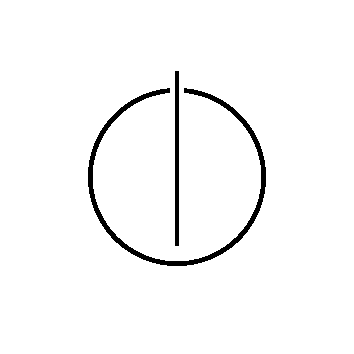
\includegraphics[width=4cm]{styles/informat.png}
  \end{figure}
  
  \end{center}
%	\clearemptydoublepage
%	
%	% The titlepage for the CAMP report document.
% Included by MAIN.TEX


%--------------------------------------------------
% The title page
%--------------------------------------------------

% correct BCOR - undo at the end !!!
\def\bcorcor{0.15cm}
\addtolength{\hoffset}{\bcorcor}

\thispagestyle{empty}

 \vspace{10mm}
\begin{center}
	       \oTUM{4cm}
	   
	   \vspace{5mm}     
	   \huge FAKULT{\"A}T F{\"U}R INFORMATIK\\ 
	   \vspace{0.5cm}
	 \large DER TECHNISCHEN UNIVERSIT{\"A}T M{\"U}NCHEN\\
        
	\end{center}
		

\vspace{10mm}
\begin{center}

   {\Large \doctype}

  \vspace{10mm}
  
  {\LARGE \title}\\
  
  
  \vspace{10mm}
  
  
  {\LARGE  \titleGer}\\
  
  
  \vspace{10mm}

    %\hfill
    \begin{tabular}{ll}
	   \Large Author:     & \Large \author \\[2mm]
	   \Large Supervisor:    & \Large Prof. Dr. Claudia Eckert\\[2mm]				
	   \Large Advisor:	& \Large M.Sc. Paul-Ioan Muntean\\[2mm]
	   \Large Date:       & \Large November 15, 2015
	 \end{tabular}
	 
	 \vspace{5mm}
	 
	 \begin{figure}[h!]
  \centering
   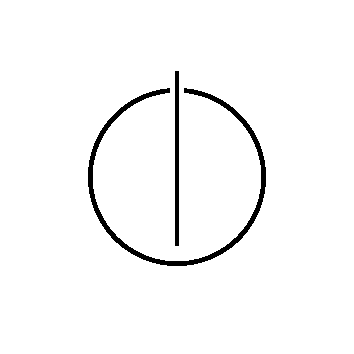
\includegraphics[width=4cm]{styles/informat.png}
  \end{figure}
   

\end{center}

% undo BCOR correction
\addtolength{\hoffset}{\bcorcor}
	
	
%	\input{components/cover_maschmeyer}
	\clearemptydoublepage
	
	% The titlepage for the CAMP report document.
% Included by MAIN.TEX


%--------------------------------------------------
% The title page
%--------------------------------------------------

% correct BCOR - undo at the end !!!
\def\bcorcor{0.15cm}
\addtolength{\hoffset}{\bcorcor}

\thispagestyle{empty}

 \vspace{10mm}
\begin{center}
	       \oTUM{4cm}
	   
	   \vspace{5mm}     
	   \huge FAKULT{\"A}T F{\"U}R INFORMATIK\\ 
	   \vspace{0.5cm}
	 \large DER TECHNISCHEN UNIVERSIT{\"A}T M{\"U}NCHEN\\
        
	\end{center}
		

\vspace{10mm}
\begin{center}

   {\Large \doctype}

  \vspace{10mm}
  
  {\LARGE \title}\\
  
  
  \vspace{10mm}
  
  
  {\LARGE  \titleGer}\\
  
  
  \vspace{10mm}

    %\hfill
    \begin{tabular}{ll}
	   \Large Author:     & \Large \author \\[2mm]
	   \Large Supervisor:    & \Large Prof. Dr. Claudia Eckert\\[2mm]				
	   \Large Advisor:	& \Large M.Sc. Paul-Ioan Muntean\\[2mm]
	   \Large Date:       & \Large November 15, 2015
	 \end{tabular}
	 
	 \vspace{5mm}
	 
	 \begin{figure}[h!]
  \centering
   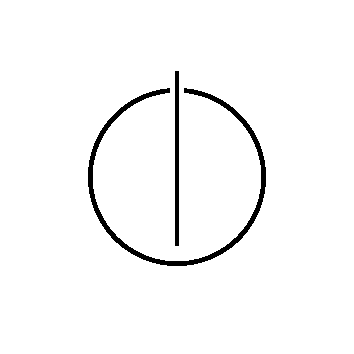
\includegraphics[width=4cm]{styles/informat.png}
  \end{figure}
   

\end{center}

% undo BCOR correction
\addtolength{\hoffset}{\bcorcor}
	
	
	\clearemptydoublepage


\thispagestyle{empty}
\selectlanguage{german}
	\vspace*{0.8\textheight}
	\noindent
	Ich versichere, dass ich diese Diplomarbeit selbst{\"a}ndig verfasst und nur 
	die angegebenen \\Quellen und Hilfsmittel verwendet habe.
	
	\vspace{15mm}
	\noindent
	M{\"u}nchen, den \today \hspace{5cm} \author
\selectlanguage{english}
\newpage
	
	\clearemptydoublepage
\phantomsection
\addcontentsline{toc}{chapter}{Acknowledgements}	


%\chapter*{Acknowledgements}

\vspace*{2cm}

\begin{center}
{\Large \bf Acknowledgments}
\end{center}

\vspace{1cm}




I would like to express my deepest appreciation to all those who provided me the possibility to complete this thesis. A special gratitude and thanks I give to my supervisor Prof. Dr. Claudia Eckert and my advisor, MSc. Paul Muntean, whose guidance, stimulating suggestions and encouragement, helped me in all the time of research and writing of this thesis. Without their cooperation in the last 6 months, this thesis could not be done smoothly.

Last but not the least, I wish to thank my family for their support and encouragement throughout my Master study.
	
	% Abstract for the TUM report document
% Included by MAIN.TEX


\clearemptydoublepage
\phantomsection
\addcontentsline{toc}{chapter}{Abstract}	





\vspace*{2cm}
\begin{center}
{\Large \bf Abstract}
\end{center}
\vspace{1cm}

Information flow vulnerabilities detection with static code analysis techniques is challenging because code
is usually not available during the software design phase and
previous knowledge about what should be annotated and tracked
is needed. To detect information flow errors in UML state
charts and C code are not easy task as they can cause data leakages or unexpected program behavior. In this research it is proposed that textual annotations used to
introduce information flow constraints in UML state charts and code which are afterwards automatically loaded by information flow checkers that check if imposed constraints hold or not. The experimental results on selected sample scenarios shows that this approach
is effective and can be further applied to other types of UML
models and programming languages as well, in order to detect
different types of vulnerabilities.

The contributions of this thesis is the development of a system for semi-automated detection of sanitization, authentication and declassification errors in UML state charts. A light-weight security annotation language is used in order to define information flow constraints regarding authentication, declassification and santization function errors  in UML state charts and source code.  Annotation language editor is designed as eclipse
plug-ins which is used to edit UML state charts and
source code files. Developed Source code generator as eclipse plug-in which is used to generate C code with header files from UML State chart. And finally experimented automatic loading and usage of textual annotations inside 3 new checkers.

	\tableofcontents
	
	\listoffigures
	
	\listoftables
  
  \clearemptydoublepage

\phantomsection
\addcontentsline{toc}{chapter}{Outline of the Thesis}

\begin{center}
	\huge{Outline of the Thesis}
\end{center}


%--------------------------------------------------------------------
%\section*{Part I: Introduction and Theory}

\noindent {\scshape Chapter 1: Introduction}  \vspace{1mm}

\noindent  This chapter presents an overview of the thesis and it's purposes. 

\noindent {\scshape Chapter 2: Background}  \vspace{1mm}

\noindent  This chapter describes the background informations and the essential theories needed for our research. Authentication, declassification and sanitization functionalities are also presented with example in this chapter. Scientific fundamentals 

%--------------------------------------------------------------------
%\section*{Part II: Implementation and Analysis}

\noindent {\scshape Chapter 3: Challenges and Annotation Language Extension}  \vspace{1mm}

\noindent  This chapter presents the challenges and annotation language extension for the system. Annotation language extension process, what technology and tools are used to develop and how it works are also presented inside this chapter.

\noindent {\scshape Chapter 4: Implementation}  \vspace{1mm}

\noindent  This chapter presents the implementation of the system. Implementation mechanism, technology and tools which have been used to develop the system are also presented inside this chapter.

\noindent {\scshape Chapter 5: Experiments}  \vspace{1mm}

\noindent  This chapter presents the different application areas of the system. Inside this chapter the system is checked for three real-life scenarios and presented the outcome of the system. 

\noindent {\scshape Chapter 6: Related Work}  \vspace{1mm}

\noindent  This chapter presents some of the related work of this research. Some of the related tools that have been already developed and comparison with them are also presented inside this chapter.


%--------------------------------------------------------------------
%\section*{Part III: Conclusion and Future Works}

\noindent {\scshape Chapter 7: Limitations, Conclusion and Future Work}  \vspace{1mm}

\noindent  This chapter presents the limitations of this research, conclusion of the whole research along with future work intentions.

	\mainmatter
	
	
		% ---------------------------------------------------------------------------
		%
		%Introduction and Background Theory
		%
		% ---------------------------------------------------------------------------
		\part[Introduction and Theory]{Introduction and Theory}
		\label{part:introAndBackgroundTheory}
		\chapter{Introduction}
\label{chapter:Introduction}

The detection of information flow vulnerabilities uses dynamic analysis techniques , static analysis techniques and hybrid techniques which combine static and dynamic approaches. The static techniques need to know when to use  sanitization , declassification and authentication functions.
A solution for tagging sanitization, declassification and authentication in source code is based on libraries which contain all needed annotations attached to function declarations. This approach plays an important role mainly for static analysis bug detection techniques where the information available during program run-time is not available nor the interaction with the environment can be fully simulated.
Extended Static Checking (ESC) is a promising research area which tries to cope with the shortage of not having the program run-time information. During extended static analysis additional information is provided to the static analysis process. This information can be used to define trust boundaries and tag variables. Textual annotations are usually manually added by the user in source code. At the same time annotations can be automatically generated and inserted into source code . ESC can be used to eliminate bugs in a late stage of the software project when code development is finished. Tagging and checking for information exposure bugs during the design phase would eliminate the potential of implementing software bugs which can only be removed very costly after wards. Thus security concerns should be enforced into source code right after the conceptual phase of the project.
The paper presents five challenges concerning ESC. The last challenge reports of the annotation as being a very time consuming burden and is therefore disliked by some programming
teams. The authors argue about the fact that annotations can cover design decisions and enhance the quality of source code. We argue that annotations are necessary in order to do ESC and the user needs a kind of assistance tool that helps selecting the suited annotation based on the current context. Thus the annotation burden needed for learning and applying the language should be reduced. At the same time adding annotations to reusable code libraries reduces even more the annotation burden since libraries can be reused, shared and changed by software development
teams.\\

Information flow errors in UML models
and code are introduced by software designers or programmers
who are sometimes blind with respect to the fact that they
are trained to focus point-wise (one code line and one data flow
at a time). This is why it is important to develop techniques
and tools which can detect this type of errors before they
materialize in production code.Information flow vulnerabilities are hard to detect because static code analysis techniques need previous knowledge about what should be considered a security issue. Code annotations which are added mainly during software development [6] can be used to provide additional knowledge regarding security
issues. On the other hand code annotations can increase the
number of source code lines by 10% [27]. In order to detect
information flow vulnerabilities software artifacts have to be
annotated with annotations attached to public data, private data and to system trust boundaries. Next, annotated artifacts have
to be made tractable by tools which can use the annotations
and check if information flow constraints hold or not based on
information propagation techniques.\\

The detection of information flow vulnerabilities in code
and UML state charts is not well addressed and is particularly
challenging. Foremost, there is no common annotation language for annotating UML state charts and source code with
information flow security constraints such that errors can be
detected also when code is not available. Second, there are
no automated checking tools which can reuse the annotated
constraints in early stages of software development to check
for information flow errors. We think that it is important to
specify security constraints as early as possible in the software
development process in order to avoid later costly repairs or
exploitable vulnerabilities.
 
\section{Latex Introduction}
There is no need for a latex introduction since there is plenty of literature out there.
 



		\chapter{Background Information}

\section{Sanitization}
Sanitization is the process of removing sensitive information from a document or other message or sometimes encrypting messages, so that the document may be distributed to a broader audience. Sometimes sanitization can be called as an operation that ensures that user input can be safely used in an SQL query. Web applications use malicious input as part of a sensitive operation without having properly checked or sanitized the input values from the user. Previous research on vulneribility analysis has mostly focused on identifying cases which web applications directly uses external input for critical operations. It is suggested that always use proper sanitization method to validate external input values from the user for any application.For example, user inputs must always flow through a sanitizing function before flowing into a SQL query or HTML, to avoid SQL injection or cross-site scripting vulnerabilities.\\

Reflection of security breaches are very significant for high assurance system. For examples of this type of systems are aircraft navigation, where a fault could lead to a crash, various control systems which has critical infrastructure , where an error 
could cause toxic waste to leak, and weapons targeting, where an inaccuracy could result in severe collateral damage. In such
operational environments, the impact is virtually irreversible and must therefore be prevented even if it is likely to occur
with low probability.It's always good that transforming information to a form which is suitable for release or sanitize the information by redacting some portions of it.\\

Three of the top five most common website attacks are SQL injection, cross-site scripting (XSS), and remote file inclusion (RFI). The root cause of these attacks is common: input sanitization. All three exploits are leveraged by data sent to the web server by the end user. When the end user is a good guy, the data he sends the server is relevant to his interaction with the website. But when the end user is a hacker, he/she can exploit this mechanism to send the web server input which is deliberately constructed to escape the legitimate context and execute unauthorized actions.\\

Input sanitization describes cleansing and scrubbing user input to prevent it from jumping the fence and exploiting security holes. But thorough input sanitization is hard. While some vulnerable sites simply don't sanitize at all, others do so incompletely, lending their owners a false sense of security.\\

Some basic purpose of sanitization are given below:
\begin{itemize}
	\item Remove malicious elements from the input.
	\item To identify the set of parameters and global variables which must be sanitized before calling functions.
	\item It is acceptable to first pass the untrusted user input through a trusted sanitization function.	
	\item Any user input data must flow through a sanitization function before it flows into a SQL query.
	\item Confidential data needs to be cleansed to avoid information leaks.
	\item Most paths that go from a source to a sink pass through a sanitizer.
	\item Developers typically define a small number of sanitization functions in libraries.
	\item Prevent web attacks using input sanitization.
\end{itemize}

\section{Declassification}
Information security has a challenge to address: enabling information flow controls with expressive information release (or declassification) policies. In a scenario of systems that operate on data with different sensitivity levels, the goal is to provide security assurance via restricting the information flow within the system. Practical security-typed languages support some form of declassification through which high-security information is allowed to flow to a low-security system or observer.\\

United States Federal Trade Commission reveals the damage that is continually caused by electronic information leakage. In protecting sensitive information, including everything from credit card information to military secrets to personal, medical information, there is a highly
need for software applications with strong, confidentiality guarantees.
Security-typed languages promise to be a valuable tool in making provably secure software applications. In such languages, each
data item is labeled with its security policy. In practical security-typed languages support some form of declassification, in which high-security information is permitted to flow to a low-security receiver/observer \\

To declassify information means lowering the security classification of selected information. Sabelfeld and Sands \cite{ref_3_sabelfeld2009declassification} identify four different dimensions of declassification, what is declassified, who is able to declassify, where the declassification occurs and when the declassification takes place.\\

Myers and Liskov introduced the decentralized label model \cite{ref_4_myers2000protecting}, describing how labels could be applied
to a programming language and then used to check information
flow policy compliance in distributed systems. The framework
includes a declassify function for downgrading data if the
owners policies allow. The model allows principals to define their own downgrading policies.\\

\subsection{Dimensions of declassification}
Classification of the basic declassification goals according to four axes: what information is released, who releases information, where in the system information is released and when information can be released.

\begin{itemize}
   \item What : Selective or Partial information flow policies \cite{ref_5_cohen1977information,ref_6_cohen1978information,ref_7_joshi2000semantic,ref_8_giacobazzi2005adjoining} regulate what
   information may be released. Partial release guarantees that only a part of a secret is
   released to a public domain. Partial release can be specified in terms of precisely which
   parts of the secret are released. This is useful,
   for example, when partial information about a credit card number or a social security number is used for logging.
   
   \item Who : In a computing system it is essential to specify who controls information release .
   Ignoring the issue of control opens up attacks where the attacker hijacks release
   mechanisms to launder secret information. Myers and Liskov decentralised label
   model \cite{ref_9_myers1997decentralized} security labels with explicit ownership information. According to this approach, information release of some data is safe if it is performed by the
   owner who is explicitly recorded in the data security label. This model has been used for enhancing Java with information flow controls \cite{ref_10_myers1999jflow} and has been implemented in
   the Jif compiler \cite{ref_11_myers2001jif}.
   
   \item Where : In a system information  Where is an important aspect of information release.One can ensure that no other  part can release further information.
   by delegating particular parts of the system to release information.Declassification
   via encryption is not harmful as long as the program is, in some sense, noninterfering
   before and after encryption.  A combination of \enquote{where} and \enquote{who} policies in the presence of encryption has
   been recently investigated by Hicks et al.\cite{ref_12_hicks2005declassification}
   
   \item When : The fourth dimension of declassification is  \enquote{when} information should be released.The work of Giambiagi and Dam \cite{ref_19_giambiagi2003secure} focuses on the correct implementation of security protocols. Here the goal is not to prove a noninterference property of the protocol, but to use the components of the protocol description as a specification of what and when information may be released.Chong and Myers security policies \cite{ref_13_chong2004security} address when information is released.By annotating variables this is achieved.
   
\end{itemize}

For a given model, the \enquote{what} and \enquote{when} dimensions seem relatively straightforward to define formally. The \enquote{what} dimension abstracts the extensional semantics
of the system; the \enquote{when} dimension can be distinguished from this since it requires an intensional semantics that (also) models time, either abstractly in terms of complexity
or via intermediate events in a computation. The \enquote{who} and \enquote{where} dimensions are
harder to formalize in a general way, beyond saying that they cannot be captured by the
\enquote{what} and \enquote{when} dimensions.

\section{Authentication}
Authentication is the mechanism which confirms the identity of users trying to access a system. For a user to be granted access to a resource, they must first prove that they are who they claim to be. Generally this is handled by passing a key with each request (often called an access token, User verification using user id and password). The system or server verifies that the access token or user id and password is genuine, that the user does indeed have the required privileges to access the requested resource and only then the request granted.\\
Also authentication can be defined as it is the process by which the system validates a user's logon information. A user's name and password are compared to an authorized list and if the system detects a match then access is granted to the extent specified in the permission list for that user.\\

One familiar use of authentication and authorization is access control. A computer system that is supposed to be used only by those authorized must attempt to detect and exclude the unauthorized. Common examples of access control involving authentication include:
\begin{itemize}	
	\item A computer program using a blind credential to authenticate to another program.
	\item Logging in to a computer.	
	\item Using an Internet banking system.
	\item Withdrawing cash from an ATM and more
	\item Assurance of identity of person or originator of data.
\end{itemize}

 A variety of authentication technologies have hit the market over the years.To better understand what they are and how they compare to the user name/password combination, it helps to be familiar with the standard authentication factors something you know, something you have and something you are and how each technology leverages them to power its authentication capabilities.
 \begin{itemize}	
	\item Something you know is a bit of knowledge committed to memory, such as a password or
	 an answer to a secret question.
	\item Something you have is an item that is owned or carried, such as a smart card or similar
	 hardware device.
	\item	 Something you are is a physical attribute that can be identified, such as a fingerprint or voice.
\end{itemize}

According to the networkworld \cite{ref_21_networld} now-a-days seven strong authentication methods are:
\begin{itemize}
\item Computer recognition software.
\item Biometrics
\item E-mail or SMS one-time password (OTP).
\item One Time Password (OTP) token.
\item Out of band.
\item Peripheral device recognition.
\item Scratch-off card.
\end{itemize}	


\section{ Detecting Information Flow Errors During Design:}
If a step of function call like authentication, sanitization or declassification is missing inside the program then this can lead to software vulnerabilities. In the figure \ref{figure_FunctionCallMissing} left side picture depicted that it has three functions. Among them func2() is named either sanitization/declassification/authentication function. Which means in this scenario there will be no error regarding sanitization/declassification/authentication function. On the other hand the right side picture represents there is a missing function of sanitization/declassification/authentication function. That's why it is the buggy path of UML state charts during design stage of software life cycle. 
\begin{figure}[htbp]
	\centering
	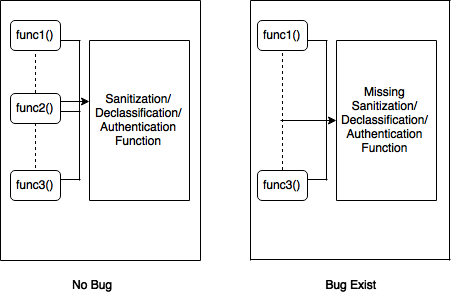
\includegraphics{styles/FunctionCallMissing.png}
	\caption{Information flow errors during design}
	\label{figure_FunctionCallMissing}
\end{figure}


\section{ Detecting Information Flow Errors During Coding:}

Figure \ref{figure_bug_detection_during_coding} depicts two explicit information flows according to A lattice model of secure information flow of Denning \cite{ref_14_denning1976lattice} contained in two systems (system 1) and (system 2)
where each of the flows starts with statement variable a and ends with leaving the system. The the variable declaration up to outside the system represent C language statements. System 1 is depicted in left side containing the flow from the source to the sink and leaving the system indicated with circles at the top and bottom of each of the
two information flows. A source is any function or programming language statement which provides private information through a system boundary. A sink can be a function call or programming language statement which exposes private information to the outside of the system through a system boundary. A system boundary can be a statement, function call, class, package or module. In figure 2.2 the source and sink represent C language statements where information enters and respectively leaves system 1 or system 2. The variable a was tagged with label \enquote{H} (confidential) as it inserts confidential information into system 1. The arrows represent the passing of the confidential label \enquote{H} between the program statements. When a variable labeled with \enquote{H} is about to leave system 1 or system 2 without passing through either authentication/declassifiaction/sanitization function then a bug report should be created.In figure 2 right side system has a bug because it passes a secured/confidential information without passing through authentication/declassifiaction/sanitization function. These functions either authenticated,declassified or sanitized  secured/confidential information and makes the variable label as \enquote{L} to leave the system. But in the left part of the picture there is no bug as in this system, secured/confidential information and the variable which is labeled with \enquote{H} passes through either authentication/declassifiaction/sanitization function.

\begin{figure}[htbp]
	\centering
	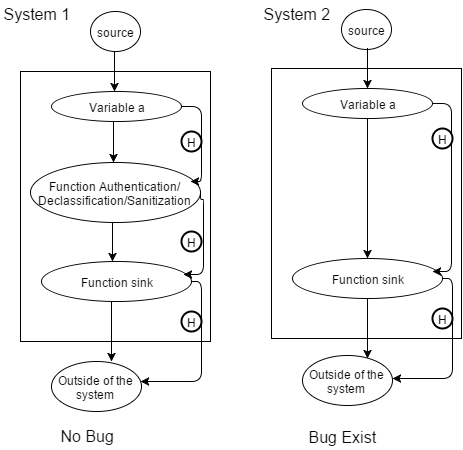
\includegraphics{styles/bug_detection_during_coding.png}
	\caption{Information flow errors during coding}
	\label{figure_bug_detection_during_coding}
\end{figure}

		
		
		
		%
		%% ---------------------------------------------------------------------------
		%%
		%% Fully Automated Calibration for Ultrasound
		%%
		%%% ---------------------------------------------------------------------------
		\part[The 2nd Part]{The Second Part}
		\label{part:secondP}
		\chapter{ Challenges and Annotation Language Extension}
Main goal is to overcome the challenge of not being able
to detect implicit and explicit information flow bugs in UML state charts and C code. An annotation language
which can be used to annotate UML state charts and code by inserting information flow
restrictions during two software development phases (design
and coding). The insight is that the same annotation language can be used to add information flow constraints to UML state charts and code in order to detect information flow errors.
 
In this chapter the challenges and how the annotation language has extended are described.

\section{Challenges and Idea}

To develop the system eclipse xtext, eclipse xtend and static analysis engine named smtcodan(which is developed in Java to detect C and C++ vulneribilities) are used. For building the source code annotation editor eclipse xtext is used. To model the source code as UML Statechart opensource platform YAKINDU SCT editor is used. Inside YAKINDU sct eclipse xtend is used mainly for genrating source code files (.c and .h files) from statechart. Below in briefly what is xtext, xtend and how it works are described.

\begin{itemize}	
	\item Xtext : Xtext is a framework for development of programming languages and domain specific languages. According to the \cite{ref_17_xtext:grammar}, it covers all aspects of a complete language infrastructure, from parsers, over linker, compiler or interpreter to fully-blown top-notch Eclipse IDE integration. It comes with great defaults for all these aspects which at the same time can be easily tailored to individual user needs.
	
	Here is an example of xtext code:
		\begin{lstlisting} [caption={Xtext Code Example},label=lst:xtextCodeExample]
		grammar org.xtext.example.mydsl.MyDsl with 
		org.eclipse.xtext.common.Terminals
		
		generate myDsl "http://www.xtext.org/example/mydsl/MyDsl"
		
		Model:
		messages+=Message*;
		
		Message:
		'Hello' name=ID '!';
		
		\end{lstlisting}
		 
	The above language allows user to write down a list of messages. The following would be the proper input messages which are allowed to write:
		\begin{lstlisting}
			Hello User!
			Hello World!		
		\end{lstlisting}
		
	\textbf{How Xtext Works:}
	Xtext provides user with a set of domain-specific languages and modern APIs to describe the different aspects of user's programming language. Based on that information it gives user a full implementation of that language running on the JVM. The compiler components of user's language are independent of Eclipse or OSGi and can be used in any Java environment. They include such things as the parser, the type-safe abstract syntax tree (AST), the serializer and code formatter, the scoping framework and the linking, compiler checks and static analysis validation and last but not least a code generator or interpreter. These runtime components integrate with and are based on the Eclipse Modeling Framework (EMF), which effectively allows user to use Xtext together with other EMF frameworks like for instance the Graphical Modeling Project GMF.
	
	In addition to this nice runtime architecture, user will get a full blown Eclipse-IDE specifically tailored for user's language. It already provides great default functionality for all aspects and again comes with DSLs and APIs that allow to configure or change the most common things very easily. And if that's not flexible enough there is Guice to replace the default behavior with user's own implementations.
	
	\textbf{Domain-Specific Language:}
	A Domain-Specific Language (DSL) is a small programming language, which focuses on a particular domain. Such a domain can be more or less anything. The idea is that its concepts and notation is as close as possible to what you have in mind when you think about a solution in that domain. 
		
	The opposite of a DSL is a so called GPL, a General Purpose Language such as Java or any other common programming language. With a GPL user can solve every computer problem, but it might not always be the best way to solve it.
	
	Imagine a user want to remove the core from an apple. User could of course use a Swiss army knife to cut it out and this is reasonable if user have to do it just once or twice. But if user need to do that on a regular basis it might be more efficient to use an apple corer.
	
	There are a couple of well-known examples of DSLs. For instance SQL is actually a DSL which focuses on querying relational databases. Other DSLs are regular expressions or even languages provided by tools like MathLab. Also most XML languages are actually domain-specific languages. The whole purpose of XML is to allow for easy creation of new languages. Unfortunately, XML uses a fixed concrete syntax, which is very verbose and yet not adapted to be read by humans. Into the bargain, a generic syntax for everything is a compromise.
	
	Xtext is a sophisticated framework that helps to implement user's very own DSL with appropriate IDE support. There is no such limitation as with XML, users are free to define users concrete syntax as users like. It may be as concise and suggestive as possible being a best match for your particular domain. The hard task of reading your model, working with it and writing it back to your syntax is greatly simplified by Xtext.
	
	\textbf{Users of Xtext:}
	Xtext is used in many different industries. It is used in the field of mobile devices, automotive development, embedded systems or Java enterprise software projects and game development. People use Xtext based languages to drive code generators that target Java, C, C++, C sharp, Objective C, Python, or Ruby code. Although the language infrastructure itself runs on the JVM, user can compile Xtext languages to any existing platform. Xtext based languages are developed for well known Open-Source projects such as Maven, Eclipse B3, the Eclipse Webtools platform or Google's Protocol Buffers and the framework is also widely used in research projects.
	
	\item Xtend : According to \cite{ref_20_xtend}, Xtend is a statically-typed programming language which translates to comprehensible Java source code. Syntactically and semantically Xtend has its roots in the Java programming language but improves on many aspects such as- Extension methods, Lambda Expressions, Active Annotations, Operator overloading, Powerful switch expressions, Multiple dispatch, Template expressions etc. Xtend has zero interoperability issues with Java: everything users write interacts with Java exactly as expected. At the same time Xtend is much more concise, readable and expressive. Its small library is just a thin layer that provides useful utilities and extensions on top of the Java Development Kit (JDK). 
	
	\textbf{Java Interoperability:}
	Xtend, like Java, is a statically typed language. In fact it completely supports Java's type system, including the primitive types like int or boolean, arrays and all the Java classes, interfaces, enums and annotations that reside on the class path.
	
	Java generics are fully supported in xtend. User can define type parameters on methods and classes and pass type arguments to generic types just as users are used to from Java. The type system and its conformance and casting rules are implemented as defined in the Java Language Specification.
	
	Resembling and supporting every aspect of Java's type system ensures that there is no impedance mismatch between Java and Xtend. This means that Xtend and Java are 100\% interoperable. There are no exceptional cases and user does not have to think in two worlds. User can invoke Xtend code from Java and vice versa without any surprises or hassles. As a bonus, if user know Java's type system and are familiar with Java's generic types, user already know the most complicated part of Xtend.
	
	The default behavior of the Xtend to Java compiler is to generate Java code with the same language version compatibility as specified for the Java compiler in the respective project. This can be changed in the global preferences or in the project properties on the Xtend  Compiler page (since 2.8). Depending on which Java language version is chosen, Xtend might generate different but equivalent code. For example, lambda expressions are translated to Java lambdas if the compiler is set to Java 8, while for lower Java versions anonymous classes are generated.
	
	\textbf{Type Inference:}
	One of the problems with Java is that you are forced to write type signatures over and over again. That is why so many people do not like static typing. But this is in fact not a problem of static typing but simply a problem with Java. Although Xtend is statically typed just like Java, user rarely have to write types down because they can be computed from the context.
	
	Consider the following Java variable declaration:
	\begin{lstlisting}
		final LinkedList<String> list = new LinkedList<String>();
	\end{lstlisting}
	The type name written for the constructor call must be repeated to declare the variable type. In Xtend the variable type can be inferred from the initialization expression:
	\begin{lstlisting}
		val list = new LinkedList<String>
	\end{lstlisting}
		
	Here is an example of xtend code:
	\begin{lstlisting} [caption={Xtend Code Example},label=lst:xtendCodeExample]
	package example	
	import java.util.List		
	class A {
	def greetToAll(List<String> names) {
		for(name: names) {
			println(name.helloMessage)
		}
	}
		
	def helloMessage(String name) {
		'Hello ' + name + '!'
		}
	}
	
	\end{lstlisting} 
	   
Xtend provides type inference, the type of name and the return types of the methods can be inferred from the context. Classes and methods are public by default, fields private. Semicolons are optional.
	
The example also shows the method helloMessage called as an extension method, like a feature of its first argument. Extension methods can also be provided by other classes or instances.
\end{itemize}


Previous annotation language grammer has been extended more
to detect implicit and explicit information flow bugs in UML
state charts and C code. The purpose of the same annotation language
can be used to add information flow constraints to UML state
charts and code in order to detect information flow errors.

The challenge was addressed by extending the annotation language containing textual annotations which can be used to annotate source code and UML state charts which are backward compatible. The single-line annotations have the same as previous consisting start tag "//@" and the multi-line annotations have the start tag "/*@" and the end tag "@*/" .

Some challenges throughout the approach are- converting textual
comments into annotations objects, introducing syntactically
correct annotations into files, how to use the same annotation
language in order to annotate UML state charts and source
code, dealing with scattered annotations and attaching annotations to the right function declaration or variable.

The eclipse xtext based grammar is used to parse the whole C/C++ language. The C/C++ source code file extensions (.h, .hh, .hhh, .hxx, .c, .cpp) and UML state chart annotation box (graphical boxes
which can be attached to different parts of a UML state chart diagram) can be annotated with policy language restrictions. The obtained CORE model (a one to one mapping from xtext grammar to the ECORE grammar representation) that can be reused for integrating the policy language into an UML state chart editor. Treating the annotation tags as EObjects created new possibilities for annotating
UML models. The policy language grammar has about 420 lines of code with code comments included. Source code generation is also supported by using
eclipse xtend, ANTLR and .mwe2 files. To parse other programming languages as well this annotation language parser can be used. The result is an extensible policy language and a highly reusable source code implementation as well as source code generator that can easily be used for annotating models and source files.

\section{Annotation Language Tags}
Table \ref{table:Security_language_annotation_tags} contains in this section: the annotation language
target types, the annotation tags which can be used in
combination with the tag @function, the tag
@parameter can be used to annotate the function parameter as authinticated/declassified/santized H/L and the tag @variable used to annotate the variable of C/C++ code with confiential H/L which are used to tag public and private variables. The tag @variable which can be used only inside single line annotations whereas @parameter is used only in multi line annotations. The tags were
defined and implemented iteratively based on the work flow
presented in figure \ref{figure:Language_Design_Process} and by using the eclipse xtext \cite{ref_17_xtext:grammar} language
definition grammar.

For detecting of authentication, declassification and sanitization errors new function tags included like authentication, declassification and sanitization function type. Also for parameter new tag type of parameter included such as authenticated, declassified and sanitized. Still H/L tags for parameter exists in the annotation tags for parameter to define that which type of parameter is this either \enquote{High} or \enquote{Low}. High means that this parameter is highly confidential or secured and low means that this parameter is not highly secured. The tag preStep used to annotate the previous function call name and tag postStep is used for next function call name. In Table \ref{table:Security_language_annotation_tags} the new tags for annotation language grammar has given with previous \cite{ref_108_paul2015infoflow} annotation tags. 

\begin{table}
	\centering
\begin{tabular}{|l|c|p{5cm}|}
	\hline
	Annotation Type   & Annotation Tag & Description  \\
	\hline

	@function         & sink  		   & uses information \\
	                  & source         & source provides information	\\
	                  & authentication & authentication is responsible for authenticate information	\\
	                  & declassification& declassification mainly declassifies information	\\
	                  & sanitization   & sanitization mainly sanitizes information	\\
	                  & trust\_boundary& trust\_boundary is a trust-boundary\\ \hline

	@parameter        & authenticated H/L& authenticated with High/Low tags\\
					  & declassified H/L  & declassified-High/Low tags    \\
				      & sanitized H/L     & sanitized with High/Low tags    \\ \hline
	@variable         & confidential H/L & confidential with High/Low tags\\
					  & source H/L & source with High/Low tags   \\
	\hline
	
	@preStep         & preStep  & previous function call name\\ 	\hline
	@postStep        & postStep  & next function call name\\ 	\hline

	
\end{tabular}
\caption{Security language annotation tags}
\label{table:Security_language_annotation_tags}
\end{table}

\section{Annotation Language Implementation Process}

To implement the annotation language Eclipse Xtext \cite{ref_17_xtext:grammar} was used. Xtext is a sophisticated framework that helps to implement own DSL (Domain Specific Language) with appropriate IDE support. There is no such limitation as with XML, users are free to define users concrete syntax as users like. It may be as concise and suggestive as possible being a best match for users particular domain. The hard task of reading user model, working with it and writing it back to users syntax is greatly simplified by Xtext. Xtext relies heavily on Eclipse Modeling Framework (EMF) internally, but it can also be used as the serialization back-end of other EMF-based tools.  

Xtext provides a lot of generic implementations for language's infrastructure but also uses code generation to generate some of the components. Those generated components are for instance the parser, the serializer, the inferred Ecore model (if any) and a couple of convenient base classes for content assist etc. The generator also contributes to shared project resources such as the plugin.xml, MANIFEST.MF and the Guice modules. Xtext's generator uses a special DSL called MWE2 - the modeling workflow engine to configure the generator. MWE2 allows to compose object graphs declaratively in a very compact manner. The nice thing about it is that it just instantiates Java classes and the configuration is done through public setter and adder methods as one is used to from Java Beans encapsulation principles.

Xtext itself and every language infrastructure developed with Xtext is configured and wired-up using dependency injection. Xtext may be used in different environments which introduce different constraints. Especially important is the difference between OSGi managed containers and plain vanilla Java programs. To honor these differences Xtext uses the concept of ISetup (src)-implementations in normal mode and uses Eclipse's extension mechanism when it should be configured in an OSGi environment.

The Modeling Workflow Engine 2 (MWE2) is a rewritten backwards compatible implementation of the Modeling Workflow Engine (MWE). It is a declarative, externally configurable generator engine. Users can describe arbitrary object compositions by means of a simple, concise syntax that allows to declare object instances, attribute values and references. One use case - that's where the name had its origins - is the definition of workflows. Such a workflow consists usually of a number of components that interact with each other. There are components to read EMF resources, to perform operations (transformations) on them and to write them back or to generate any number of other artifacts out of the information. Workflows are typically executed in a single JVM. However there are no constraints that prevent implementors to provide components that spawn multiple threads or new processes.

Xtext ships with a default set of predefined, reasonable and often required terminal rules. The grammar for these common terminal rules is defined as follows:
	\begin{lstlisting}[caption={Common terminal Rules in Xtext },label=lst:xtextCommonTerminalRules]
		grammar org.eclipse.xtext.common.Terminals 
		hidden(WS, ML_COMMENT, SL_COMMENT)
		import "http://www.eclipse.org/emf/2002/Ecore" as ecore
		terminal ID : 
		'^'?('a'..'z'|'A'..'Z'|'_')('a'..'z'|'A'..'Z'|'_'|'0'..'9')*;
		terminal INT returns ecore::EInt: 
		('0'..'9')+;
		terminal STRING  : 
		'"' ( '\\'('b'|'t'|'n'|'f'|'r'|'u'|'"'|"'"|'\\') | !('\\'|'"') )* '"' |
		"'" ( '\\'('b'|'t'|'n'|'f'|'r'|'u'|'"'|"'"|'\\') | !('\\'|"'") )* "'"; 
		terminal ML_COMMENT  : 
		'/*' -> '*/';
		terminal SL_COMMENT : 
		'//' !('\n'|'\r')* ('\r'? '\n')?;
		terminal WS  : 
		(' '|'\t'|'\r'|'\n')+;
		terminal ANY_OTHER: 
		.;
	\end{lstlisting}

In order to implement the annotation language grammer in this research it was required to extend the terminal rule ML\_COMMENT and SL\_COMMENT. After extending these two rules it looks like this:

\begin{lstlisting}[caption={Sigleline and Multiline Comments Rule in Xtext},label=lst:slMlRuleXtext]
	/**
	* @SL_COMMENT :all strings which follow // | || | } will be a single line comment
	*/ 
	terminal SL_COMMENT 	: '//'!('@')  !('\n'|'\r')* ('\n'|'\r')*
	// '}' can be used optional to disable the method bodyes together with multiline line {} comment 
	//     | '}'         !('\n'|'\r')* ('\n'|'\r')*               
	;
	
	/**
	* @ML_COMMENT :@/* multiline comment excluding @ from inside
	*            :{} multi line comment 
	*/ 
	terminal ML_COMMENT	: '/*' !('@') -> !('@')'*/'   !('\n'|'\r')* ('\n'|'\r')*   
	// '{' -> '}' can be used optional to disable the method bodies together with single line { comment 
		//      | '{' -> '}'                   ('\n'|'\r')?
		;   
\end{lstlisting}

The process depicted in figure \ref{figure:Language_Design_Process} was used in order to
implement annotation language. The process is
comprised of the following steps: At first, the .xtext file
containing the language grammar was extended following the requirements. Next the grammar file is compiled and software artifacts are generated. After editing the .mwe2 file then need to compile it. The result of compiling is: a parser, a lexer and class bindings between these two (lexer and parser) and the grammar ECore model. The generated parser, lexer and the bindings were reused inside static analysis engine and in the UI source file editor. After opening and editing a source file with the editor, the file can be parsed and the annotations can be automatically loaded and used inside checkers.
\begin{figure}[htbp]
	\centering
	\makebox[\textwidth]{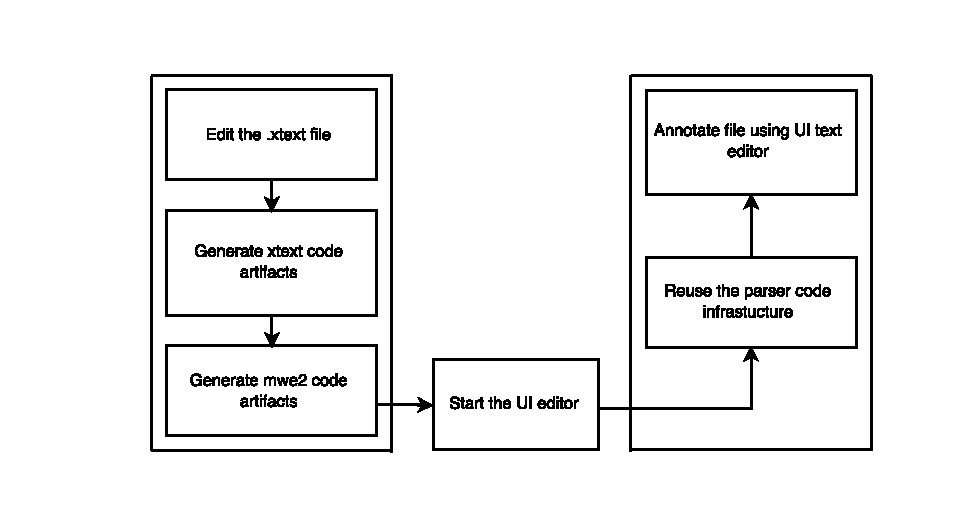
\includegraphics[width=\textwidth,scale=.50]{styles/Language_Design_Process.pdf}}
	\caption{Annotation language design process}
	\label{figure:Language_Design_Process}
\end{figure}
		\chapter{Implementation}
This chapter focus mainly about the software implementation for semi-automated detection of sanitization, authentication and declassification errors in UML state Charts. Used Eclipse xtext to develop source code editor, Eclipse xtend to develop source code generator, YAKINDU SCT editor for modeling C/C++ programs as UML statchart and extended static analysis engine named smtcodan using Java, Graphics2D and Jframe. 

\section{Overview of System Architecture}

A system architecture or systems architecture is the conceptual model that defines the structure, behavior and more views of a system. An architecture description is a formal description and representation of a system, organized in a way that supports reasoning about the structures and behaviors of the system.

It can be said that the system architecture is (similar to the one of a building architecture)  a global model of this system consisting of:
\begin{itemize}
	\item   a structure
	\item	properties (of various elements involved)
	\item	relationships (between various elements)
	\item	behaviors and dynamics
	\item	multiple views of the system (complementary and consistent).
\end{itemize}

System Architecture is based on 9 fundamental principles:
\begin{itemize}
	\item The objects of the reality are modeled as systems
	\item A system can be broken down into a set of smaller subsystems, which is less than the whole system
	\item A system must be considered in interaction with other systems
	\item A system must be considered through its whole lifecycle
	\item System can be linked to another through an interface, which will model the properties of the link
	\item A system can be considered at various abstraction levels, allowing to consider only relevant properties and behaviors
	\item A system can be viewed according to several layers (usually three: its sense, its functions, and its composition)
	\item A system can be described through interrelated models with given semantics (properties, structure, states, behaviors, datas, etc)
	\item A system can be described through different viewpoints corresponding to various actors concerned by the system.
\end{itemize}

The architecture of our system is given below:
\begin{figure}[htbp]
	\centering
	\makebox[\textwidth]{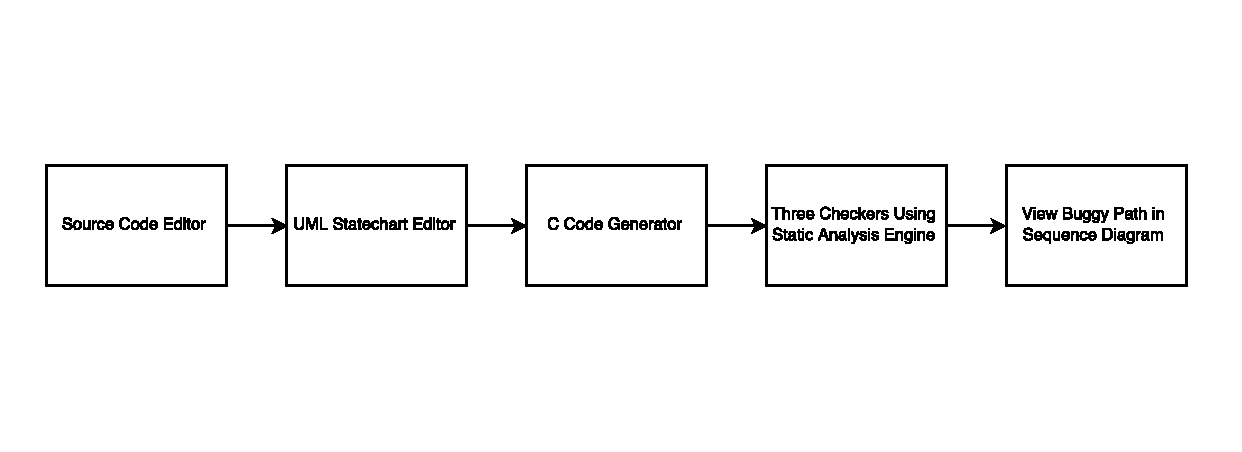
\includegraphics[scale=.50,width=\textwidth]{styles/system_architecture.pdf}}
	\caption{System Overview}
	\label{system_architecture}
\end{figure}

Figure \ref{system_architecture} depicts the complete system overview. First which is presented as number \textcircled{1}, the source code editor is developed using Eclipse Xtext. By this editor one can easily annotate the source code of C/C++. Even it is possible to annotate C/C++ header files. For information flow vulnerabilities detection in C/C++ code this annotation technique has chosen which is easy to extend and backward compatible. This editor has developed as an Eclipse plug-in. If this plug-in exist in eclipse then user can easily annotate C/C++ source code files and header files by pressing the keys ctrl+space in keyboard. Then for modeling purpose open source tool Yakindu SCT editor \cite{ref_15_yakindu:sct} has chosen to model the C/C++ code into state charts to detect the bug during design stage of software development life-cycle which is depicted as number \textcircled{2} in the figure \ref{system_architecture}. Inside the Yakindu SCT editor the annotation language grammar has also included using Eclipse Xtext. So, that user can easily annotate the state charts to detect the information flow vulnerabilities. Afterwards the C code generator has extended inside the Yakindu SCT editor using Eclipse Xtend. This C code generator is represented as number \textcircled{3} in the figure \ref{system_architecture}. After modeling the C code files in Yakindu SCT editor user can easily generate the code using C code generator. Through this generator two files will be generated. One file has .c extension and another file has .h extension. Inside those files annotation has also included. Those annotations are helpful to detect the information flow errors. After generating the code files using static analysis engine named \enquote{smtcodan} three checkers have included to detect authentication, declassification and sanitization function missing vulnerabilities. This three checkers have represented as number \textcircled{4} phase in the figure \ref{system_architecture}. Inside the static analysis engine according to the requirements new modules are added. Then to view the buggy path in sequence diagram a sequence diagram generator has created. Sequence diagram generator to view buggy path is the number \textcircled{5} and last phase of the system. That is the end of complete system architecture of this system. 


\section{The Grammar of Annotation Language}

The goal of the annotation language is to convey library-specific information to the compiler in a simple declarative manner. While it's clear that more sophisticated specifications could support more sophisticated optimizations, our goal is to show that a few simple annotations can enable many useful optimizations. Simplicity is important because we expect our language users to be library experts who do not necessarily have expertise in compilers or formal specifications.

An annotation is metadata (like a comment, explanation, presentational markup) attached to text, image, or other data. Often, annotations refer to a specific part of the original data.Markup languages like XML and HTML annotate text in a way that is syntactically distinguishable from that text. They can be used to add information about the desired visual presentation, or machine-readable semantic information. If annotations are to be machine-readable, they must have a well-defined syntax, and if a tool's checks are to be meaningful, the annotations also need a well-defined semantics. Quite a few specification languages have been defined over the past several decades; 

A special case is the Java programming language, where annotations can be used as a special form of syntactic metadata in the source code. Classes, methods, variables, parameters and packages may be annotated. The annotations can be embedded in class files generated by the compiler and may be retained by the Java virtual machine and thus influence the run-time behavior of an application. It is possible to create meta-annotations out of the existing ones in Java.

The "annotate" function (also known as "blame" or "praise") used in source control systems such as Git, Team Foundation Server and Subversion determines who committed changes to the source code into the repository. This outputs a copy of the source code where each line is annotated with the name of the last contributor to edit that line (and possibly a revision number). This can help establish blame in the event a change caused a malfunction, or identify the author of brilliant code.

For example, Standard Annotation Language or SAL \cite{ref_51_microsoft:sal} is a meta-language that can help static analysis tools, such as analyze switch in Visual Studio 2005 Team System and Visual Studio 2005 Team Edition for Developers, find bugs including security bugs in your C or C++ code at compile time.
Using SAL is relatively easy. You simply add annotations to your function prototypes that describe more contextual information about the function being annotated. This can include annotations to function arguments and to function return values. The initial focus of SAL is to annotate functions that manipulate read and write buffers. In Windows Vista we are annotating all appropriate functions before the product is released to customers to help us find bugs as early as possible.

\begin{table}
	\centering
	\begin{tabular}{|l|c|p{5cm}|}
		\hline
		Category  & Parameter Annotation & Description  \\
		\hline
		
		Input to called function        & \_In\_k  		   & Data is passed to the called function, and 
		is treated as read-only\\
		\hline
		
		Input to called function, and output to caller        & \_Inout\_ & Usable data is passed into the function 
		and potentially is modified. \\ \hline
		Output to caller        & \_Out\_ & The caller only provides space 
		for the called function to write to. 
		The called function writes
		data into that space. \\
		\hline
		
		Output of pointer to caller         & \_Outptr\_  & Like Output to caller. The value that's returned by the called function is a pointer.\\ 	\hline
			
	\end{tabular}
	\caption{SAL-four basic kinds of parameters}
	\label{table:four basic kinds of parameters}
\end{table}

These four basic annotations can be made more explicit in various ways. By default, annotated pointer parameters are assumed to be required ,they must be non-NULL for the function to succeed. The most commonly used variation of the basic annotations indicates that a pointer parameter is optional, if it's NULL, the function can still succeed in doing its work.These annotations help identify possible uninitialized values and invalid null pointer uses in a formal and accurate manner. Passing NULL to a required parameter might cause a crash, or it might cause a "failed" error code to be returned. Either way, the function cannot succeed in doing its job.

The main benefit of SAL is that you can find more bugs with just a little bit of upfront work. The process of adding SAL annotations to existing code can also find bugs as the developer questions the assumptions previously made about how the function being annotated works. By this as a developer adds annotations to a function, she must think about how the function works in more detail than simply assuming it was written correctly. This process finds assumption flaws. Any bugs found in SAL annotated functions tend to be real bugs, not false positives, which has the benefit of speedier bug triage and code fixes.

In this research, annotation language is developed using Eclipse xtext \cite{ref_17_xtext:grammar}. The goal is to overcome the challenge of not being able to detect implicit and explicit information flow bugs in UML state charts and C code. That's why an annotation language has chosen
which can be used to annotate UML state charts and code by inserting information flow
restrictions during two software development phases (design
and coding). Our insight is that the same annotation language
can be used to add information flow constraints to UML state
charts and code in order to detect information flow errors. The grammar of annotation language is represented as in Extended Backus Naur Form (EBNF) in Figure \ref{language grammar}. The following type face conventions were used: Italic font for non-terminals, bold typewriter font for literal terminals including keywords.\\
 
 \begin{figure}[ht!]
 	\centering
 	\begin{tabular}{lll}
 		
 		\footnotesize                       
 		\textit{Ann\_Lang}           &\footnotesize $::=$         &\footnotesize HeaderModel*;       \\ \\
 		
 		\footnotesize
 		\textit{H\_Model}            &\footnotesize $::=$         &\footnotesize \textit{S\_L\_Anno};       \hfill ;single line comment rule   \\     
 		&\footnotesize $\ \vert $    &\footnotesize \textit{M\_L\_Anno};       \hfill ;multi line comment rule    \\ 
 		&\footnotesize $\ \vert $    &\footnotesize \textit{Func\_Ann};       \hfill ;function declaration rule  \\ 
 		&\footnotesize $\ \vert $    &\footnotesize \textit{Attr\_Def};        \hfill ;variable declaration rule  \\ \\
 		\footnotesize  	
 		\textit{S\_L\_Anno}          &\footnotesize $::=$         &\footnotesize \textbf{"//@ @function "},    Func\_Type,              [\textbf{H} $\ \vert $  \textbf{L}];     \\
 		&\footnotesize $\ \vert $    &\footnotesize \textbf{"//@ @parameter "},   p\_Name,  Sec\_Type, Var\_Type,    [\textbf{H} $\ \vert $  \textbf{L}];    \\
 		&\footnotesize $\ \vert $    &\footnotesize \textbf{"//@ @variable "},    v\_Name,  Sec\_Type,     [\textbf{H} $\ \vert $  \textbf{L}];    \\
 		&\footnotesize $\ \vert $    &\footnotesize \textbf{"//@ @preStep "},     pr\_s\_Name,             [\textbf{H} $\ \vert $  \textbf{L}];    \\
 		&\footnotesize $\ \vert $    &\footnotesize \textbf{"//@ @postStep "},    po\_s\_Name,             [\textbf{H} $\ \vert $  \textbf{L}];    \\ \\   
 		\footnotesize            
 		\textit{M\_L\_Anno}          &\footnotesize $::=$         &\footnotesize [\textbf{"/*@ "}],  ["* "],  Func\_Ann,  (\textbf{" @*/"}) \\
 		&\footnotesize $\ \vert $    &\footnotesize ("*"), [" "]*, (\textbf{"@*/"});                  \\ \\
 		\footnotesize        
 		\textit{Func\_Ann}           &\footnotesize $::=$         &\footnotesize \textbf{"@function "},    Func\_Type,              [\textbf{H} $\ \vert $  \textbf{L}];     \\
 		&\footnotesize $\ \vert $    &\footnotesize \textbf{"@parameter "},   p\_Name,  Sec\_Type, Var\_Type,    [\textbf{H} $\ \vert $  \textbf{L}];    \\
 		&\footnotesize $\ \vert $    &\footnotesize \textbf{"@preStep "},     pr\_s\_Name,             [\textbf{H} $\ \vert $  \textbf{L}];    \\
 		&\footnotesize $\ \vert $    &\footnotesize \textbf{"@postStep "},    po\_s\_Name,             [\textbf{H} $\ \vert $  \textbf{L}];    \\ \\                                        
 		\footnotesize                       
 		\textit{Func\_Type}          &\footnotesize $::=$        &\footnotesize \textbf{authentication};\\
 		&\footnotesize $\ \vert $ &\footnotesize \textbf{declassification}; \\
 		&\footnotesize $\ \vert $    &\footnotesize \textbf{sanitization};     \\
 		&\footnotesize $\ \vert $    &\footnotesize \textbf{sink};             \\
 		&\footnotesize $\ \vert $    &\footnotesize \textbf{source};           \\
 		&\footnotesize $\ \vert $    &\footnotesize \textbf{trust\_boundary};  \\ \\
 		\footnotesize                       
 		\textit{Sec\_Type}           &\footnotesize $::=$         &\footnotesize \textbf{confidential}; \\
 		&\footnotesize $\ \vert $    &\footnotesize \textbf{source};    \\ \\
 		\footnotesize                       
 		\textit{Var\_Type}           &\footnotesize $::=$         &\footnotesize \textbf{authenticated}; \\
 		&\footnotesize $\ \vert $    &\footnotesize \textbf{declassified}
 		\\
 		&\footnotesize $\ \vert $    &\footnotesize \textbf{sanitized};    \\ \\	
 		
 	\end{tabular}
 	\caption{Light-weight annotation language grammar excerpt}
 	\label{language grammar}
 \end{figure}
 
All main rules are included under \texttt{H\_Model}. This  \texttt{H\_Model} rule contains all rules like \texttt{S\_L\_Anno}, \texttt{M\_L\_Anno}, \texttt{Func\_Ann} and \texttt{Attr\_Def}. Annotation language grammar has two grammar rules named \texttt{S\_L\_Anno} and \texttt{M\_L\_Anno} used for defining security annotations. \texttt{S\_L\_Anno} is used for single line annotation rule. Because of this rule one can easily annotate the variables of C/C++ language in a single line. The \texttt{M\_L\_Anno} rule is used for multiline annotation rule. Normally multiline rule annotation is required for function annotation in C/C++ function declaration. The \texttt{Func\_Ann} and \texttt{Attr\_Definition} rules are used to recognize C or C++ function declarations and variable. The \texttt{Var\_Type} rule is used for variable type which is either for authenticated or declassified or sanitized variable. \texttt{Sec\_Type} rule is used for type of security whether a variable is confidential or not. In \texttt{Func\_Type} rule the type of function is declared. A function can be either one of this like authentication, declassification, sanitization, source or sink.\\


\section{UML State Chart Editor}

UML is a standard language for specifying, visualizing, constructing, and documenting the artifacts of software systems.UML was created by Object Management Group and UML 1.0 specification draft was proposed to the OMG in January 1997. UML provides elements and components to support the requirement of complex systems. UML follows the object oriented concepts and methodology. So object oriented systems are generally modeled using the pictorial language.UML diagrams are drawn from different perspectives like design, implementation, deployment etc. UML can be defined as a modeling language to capture the architectural, behavioral and structural aspects of a system.

UML state machine diagrams depict the various states that an object may be in and the transitions between those states. In fact, in other modeling languages, it is common for this type of a diagram to be called a state-transition diagram or even simply a state diagram. A state represents a stage in the behavior pattern of an object and like UML activity diagrams it is possible to have initial states and final states. An initial state, also called a creation state, is the one that an object is in when it is first created, whereas a final state is one in which no transitions lead out of. A transition is a progression from one state to another and will be triggered by an event that is either internal or external to the object.

Statechart diagram defines the states of a component and these state changes are dynamic in nature. So its specific purpose is to define state changes triggered by events. Events are internal or external factors influencing the system. Statechart diagrams are used to model states and also events operating on the system. When implementing a system it is very important to clarify different states of an object during its life time and statechart diagrams are used for this purpose. When these states and events are identified they are used to model it and these models are used during implementation of the system. The main usages of UML state chart are:
\begin{itemize}
	\item To model object states of a system.
	\item To model reactive system. Reactive system consists of reactive objects.
	\item To identify events responsible for state changes.
	\item Forward and reverse engineering.
\end{itemize}

\begin{figure}[htbp]
	\centering
	\makebox[\textwidth]{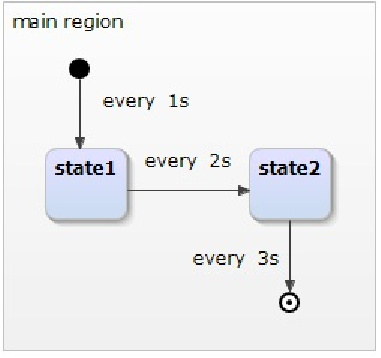
\includegraphics[width=55mm,scale=.55]{styles/simpleStateChart.pdf}}
	\label{simple_stateChart}
	\caption{Simple UML State Chart}
\end{figure}

The following are the basic notational elements that can be used to make up a diagram represented in figure \ref{simple_stateChart}:
\begin{itemize}
	\item Filled circle, representing to the initial state.	
	\item Hollow circle containing a smaller filled circle, indicating the final state (if any).	
	\item Rounded rectangle, denoting a state.	
	\item Arrow, denoting transition.	
\end{itemize}

Statechart diagram is used to describe the states of different objects in its life cycle. So the emphasis is given on the state changes upon some internal or external events. These states of objects are important to analyze and implement them accurately. Following are the main purposes of using Statechart diagrams:

\begin{itemize}
	\item To model dynamic aspect of a system.
	
	\item To model life time of a reactive system.
	
	\item To describe different states of an object during its life time.
	
	\item Define a state machine to model states of an object.
\end{itemize}

A set of formal representation of UML state charts is presented in this section. The state identifier and event are represented as S and Event respectively both as set types. For simple specification, the basic set types are used. In the definition of a transition from one state to another the guard is defined as a Boolean type. According to F Alhumaidan state based static and dynamic formal analysis of UML state diagrams \cite{ref_16_alhumaidan2012state} , a state can have three possible values that are active, passive or null represented as Active, Passive and null respectively. The type of state can be simple, concurrent, non-concurrent, initial or final.

\begin{figure}[ht!]
	\centering
	\begin{tabular}{lll}
		\footnotesize                       
		\textit{[S, Event]}          &\footnotesize \\
		
		\footnotesize
		\textit{Boolean}            &\footnotesize $::=$         &\footnotesize \textit{True} $\ \vert $ {False};       \\   
		\footnotesize
		\textit{Status}            &\footnotesize $::=$         &\footnotesize \textit{Active}
		 $\ \vert $ {Passive}$\ \vert $ {Null};       \\ 
		\footnotesize
		\textit{Type}            &\footnotesize $::=$         &\footnotesize \textit{Simple}
		 	$\ \vert $ {Concurent}$\ \vert $ {Nonconcurent} $\ \vert $ {Initial}$\ \vert $ {Final};       \\	 	 
		
	\end{tabular}
	\caption{UML Statechart Formal Representation}
	\label{statechart_formal_representation}
\end{figure}

In modeling using sets, it's not imposing any restriction upon the number of elements and a high level of
abstraction is supposed. Further, it's not insist upon any
effective procedure for deciding whether an arbitrary
element is a member of the given collection or not. As a
consequent, sets S and Event are sets over which cannot define any operation of set theory. For example,
cardinality to know the number of elements in a set cannot
be defined. Similarly, the subset, union, intersection or
complement operations over the sets are not defined.\\

The state diagram is a collection of states related by
certain types of relations. In the definition of a state, state identifier, its type, status and set of regions is required.Region is defined as a power set of sequence of states. The state is represented by a schema which consists of four components described above. All these components are encapsulated and put in the Schema State given below.
The invariants over the schema are defined in the second
part of schema.\\

\begin{figure}[ht!]
	\centering
	\begin{tabular}{lll}
		\footnotesize                       
		\textit{State}       \\
		
		\footnotesize
		\textit{name}   $:$    \textit{S}  \\   
		\footnotesize
		\textit{type}   $:$    \textit{Type}  \\   
		\footnotesize
		\textit{status}   $:$    \textit{Status}      \\
		\footnotesize
		\textit{regions} $:$   \textit{seq Regions} \\
		
		\footnotesize
		\textit{regions} $=$   \textit{1} $\ \  $ {type}$=$   \textit{Simple} \\
		\footnotesize
		 \textit{\# regions} $=$   \textit{1} $\ \  $ {type}$=$   \textit{Nonconcurrent} \\
		 \textit{\# regions} $=$   \textit{1} $\ \  $ {type}$=$   \textit{Concurent} \\
		 
		
	\end{tabular}
	\caption{UML statechart some other formal representation}
	\label{statechart_formal_representation_part2}
\end{figure}

\textbf{Invariants:}
\begin{itemize}
\item  If there is no region in a state inside the state diagram, then it is a simple state.
\item  If there is exactly one region in a state then it is termed as non-concurrent composite state.
\item  If there are two or more regions in a state then it is
concurrent composite state.
\end{itemize}

The collection of states is represented by the schema
States which consists of four variables. The mapping
sub states from State to power set of State describes type
of a state.
 \begin{figure}[ht!]
 	\centering
 	\begin{tabular}{lll}
 		\footnotesize                       
 		\textit{States}          \\
 		\footnotesize                       
 		\textit{start}          
 		$:$  \textit{State}\\
 		
 		\textit{states}          
 		$:$  \textit{State}\\
 		
 		\textit{states}           
 		$:$  \textit{State}\\
 		\footnotesize
 		\textit{substates}            $:$         \textit{State} $\ \  $ {State};       \\   
 		\footnotesize
 		\textit{target}             $:$         \textit{State}    \\
 		 \footnotesize                       
 		 \textit{start}           
 		 $:$  \textit{states}\\
 		  \footnotesize                       
 		  \textit{start}          
 		  $:$ \textit{target}\\
 		   \footnotesize                       
 		   \textit{start}           
 		   $:$  \textit{dom} $\ \  ${substates}\\
 		   
 		   \footnotesize                       
 		   \textit{states}          \\ 		
 		$\ \  $ \textit{s}      $:$     \textit{State} $\ \  $ {s} $\ \  $ \textit{dom} $\ \  ${substates} $\ \  $ {s} $\ \  $ \textit{states}        \\ 
 		$\ \  $ \textit{s}      $:$     \textit{State} $\ \  $ {s} $\ \  $ \textit{states} $\ \  $ {s} $\ \  $ \textit{start} $\ \  $ {s} $\ \  $ \textit{target}$\ \  $ {s.typ}\\ 
 		$\ \  $ \textit{Simple} $\ \  $ {s} $\ \  $ \textit{dom} $\ \  ${substates}\\
 		\footnotesize                       
 		\textit{target}  $\ \  $ \textit{states}        \\ 
 		\footnotesize                       
 		\textit{target}  $\ \  $ \textit{dom} $\ \  ${substates}\\	
 	\end{tabular}
 	\caption{UML Statechart Formal Representation some parts}
 	\label{statechart_formal_representation_invariants}
 	\end{figure}

\textbf{Invariants:}
\begin{itemize}
\item The start state is not in the collection of states.
\item The start state is not the target state.
\item The start state does not belong to domain of substates
mapping that is it has no sub-state.
\item The set of states is non-empty.
\item For any state, s, if it is in the states and is not the start or target state and not the simple state then it belongs to domain of sub-states.
\item The target state does not belong to states.
\item The target state of the state diagram does not belong to domain of the sub-states.
\end{itemize}

UML state chart editor has been extended based on the open source Yakindu SCT \cite{ref_15_yakindu:sct}framework. The existing language grammar with
annotation language grammar has extended in order to support new set
of tags. Furthermore, an annotation proposal filter implemented which was used to filter out the annotation language tags of the Yakindu SCT language grammar.\\

To extend the Yakindu SCT editor here it has been decided to represent the statements like variable declaration, function calling as state and transitions are represent as move from one statement to another. A rectangular box can be attached with transitions where annotation can be written as per requirements. So for the developed system the UML statechart formal representation is as like this: 
\begin{figure}[ht!]
	\centering
	\begin{tabular}{lll}
	\footnotesize                       
	\textit{States}          \\
	\footnotesize                       
	\textit{start}          
	$:$  \textit{State}\\
	
	\textit{states}          
	$:$  \textit{State}\\
	
	\textit{states}           
	$:$  \textit{State}\\
	\footnotesize
	\textit{substates}            $:$         \textit{State} $\ \  $ {State};       \\   
	\footnotesize
	\textit{target}             $:$         \textit{State}    \\
	\footnotesize                       
	\textit{start}           
	$:$  \textit{states}\\
	\footnotesize                       
	\textit{start}          
	$:$ \textit{target}\\
	\footnotesize                       
	\textit{transition}          
	$:$ \textit{annotation*}\\
	\footnotesize                       
	\textit{target} $:$ \textit{states}        \\ 	
	\end{tabular}
	\caption{UML Statechart Formal Representation for this System}
	\label{statechart_formal_representation_for _this_system}
	\end{figure}
\section{Source Code Editor}

A source code editor is a text editor program designed specifically for editing source code of computer programs by programmers. It may be a standalone application or it may be built into an integrated development environment (IDE) or web browser. Source code editors are the most fundamental programming tool, as the fundamental job of programmers is to write and edit source code.Source code editors have features specifically designed to simplify and speed up input of source code, such as syntax highlighting, indentation, autocomplete and bracket matching functionality. Some well-known source code editors are:
\begin{itemize}
	\item Gedit 
	\item IntelliJ 
	\item NetBeans
	\item Notepad++ and more.
\end{itemize}

The source code editor \cite{ref_108_paul2015infoflow} has extended which offers annotation language proposals which are context sensitive with respect to the position of the currently edited syntax line. Editor suggestions work only if the whole file is parsed without errors. Editor was developed using Eclipse Xtext \cite{ref_17_xtext:grammar}.

As per requirements previous annotation language grammar \cite{ref_108_paul2015infoflow} which was written in xtext language has been extended. Extra annotation have included like \enquote{authenticated}, \enquote{declassified}, \enquote{sanitized}, \enquote{sanitization}, \enquote{declassification}, \enquote{authentication}. Mainly FunctionAnnotation, FunctionType  and SingleLineAnnotation rules  are extended. A new rule is added which is enumeration type. The rule name is VariableType. Inside the VariableType new attributes are included like declassified, sanitized and authenticated. New function types are added like declassification, sanitization and authentication function inside FunctionType rule. Inside the FunctionAnnotation and SingleLineAnnotation rules there exist an annotation for parameter name @parameter. Inside @ parameter declaration new attribute is added named VariableType. The code snippet of extended xtext grammar has given in \ref{Source_Code_Editor_in_Xtext}. 


From the xtext code snippet previous annotation grammar \cite{ref_108_paul2015infoflow} has FunctionAnnotation(line number 113), SingleLineAnnotation(line number 128) rules. According to the requirements previous rules are extended. Inside the rules of FunctionAnnotation and SingleLineAnnotation new enumeration types are added. Enumeration type name is VariableType which is declared in line number 172 in \ref{Source_Code_Editor_in_Xtext}. The new enumeration type rule has attributes declassified, sanitized and authenticated. Also the rule of enumeration FunctionType(line number 154 in \ref{Source_Code_Editor_in_Xtext}) extended by adding new type of funtion like authentication, declassification and sanitization.

\section{C Code Generator}
C code generator \cite{ref_108_paul2015infoflow} has extended based on Eclipse EMF and xTend which is used to generate the state chart execution code containing the previously added security annotations from UML state charts. The code generator outputs two files per UML state chart (one .c and one
.h file). Generated annotations can reside in both header file
and source code file. Previously annotated UML state chart
states are converted to either C function calls or C variables
declarations, both have been previously annotated. We use
the available state chart execution flow functionality which is
responsible for traversing the UML state chart during state
chart simulation. The UML state chart will be traversed by the code generation algorithm and code is generated based on
the mentioned state chart execution flow. The generated code
will contain at least one bad path (contains a true positive) and
a good path (contains no bug) per UML state chart if those
paths were previously modeled inside the UML state chart.

The algorithm \ref{Algorithm:C_Code_Generator} which is given below is representing how the C code generator has been created. The input of the algorithm for code generator is UML statechart. In eclipse xtend \cite{ref_20_xtend} function can be declared as \enquote{def}. Inside the algorithm \ref{Algorithm:C_Code_Generator} the generateTypeH function requires the input of UML statechart. The plug-in named \enquote{MyC} uses eclipse xtend to parse the UML statechart. Inside this function there another two functions named \enquote{typesHAnnotationContent} to generate header file of c(extension .h) and \enquote{typesCAnnotationContent} to generate source code file of c(extension .c).Function typesHAnnotationContent generate the required contents for C header file mostly function signature and annotation of the function which exist in the UML statechart. 

One sample example of a header file is given below-

\begin{lstlisting} [caption={C Header File Codes with Annotation},label=lst:cHeaderFileCode]
	/*@ @function authentication
	* @parameter a L @*/
	void authentication(char *a);
	
	/*@ @function source
	* @parameter a L @*/
	void logIn(char *a);
\end{lstlisting}

Inside the algorithm \ref{Algorithm:C_Code_Generator} function typesCAnnotationContent generate the required contents for C source file. This file contains the annotation only for variable declaration. The function annotation is normally located at header file. In this file other code is as normal as C syntax. All functions, statements, variable declaration are similar to C programming language syntax. Inside the function typesHAnnotationContent at first need to get the function annotation as we placed the function signature and function annotation inside the header file. That's why we declared a method named getFileContent who returns a hashmap which contains annotations and statements like variable declaration and function signatures. By iterating the hashmap need to make a check if current statement is not a variable annotation then we placed the annotation and function signatures inside the C header file.

Function typesCAnnotationContent is responsible to generate the C source code. Inside this function to get all function content there is a method called getFunctionContent which returns a hashmap with all function signatures and annotation. By iterating that hashmap the required function signatures are placed inside the C code file. Those functions who has annotations only signatures and blank function bodies are placed inside the C source code file. Because the annotations of the functions mainly placed inside the header file. Now in the modeling stage the system was designed with two regions. One region name is good\_path() and another one is bad\_path(). To get the content of good\_path() and bad\_path(), two methods have created inside the Naming.xtend file named getGoodPathContent() and getBadPathContent(). Those two methods also returned two hashmaps respectively. One hashmap contains the contents of good\_path() region and another hashmap contains the contents of bad\_path() region. Both hashmaps contains the function signatures, statements of C/C++ language and annotations. According to the design in the modeling stage the required contents are placed inside the body of good\_path() and bad\_path(). Normally inside the method of good\_path() and bad\_path() only the variable annotations exist and other statement like function calling, variable declarations etc. The annotations for functions are placed inside the header files of C/C++ language. 

Some of the contents of the header file, C file comes from another xtend file named \enquote{Naming.xtend} which contains in \enquote{MyC} project folder of YAKINDU Sct Editor. the methods like getFileContent, getFunctionContent, getGoodPathContent() and getBadPathContent() all are implemented inside the "Naming.xtend" file. The code snippet from C code generator has given in \ref{C_Code_Generator_Xtend_Code_Snippet}.

\begin{algorithm}
	\label{Algorithm:C_Code_Generator}
	{\textbf{C code generator}}\\
	\noindent\makebox[\linewidth]{\rule{\textwidth}{0.4pt}}
	{\textbf{Input: Statechart}} \\
	{\textbf{Output: .c and .h files}}
	\begin{algorithmic}[1]
	
		\Function{generateTypesH}{$sc$}\Comment{Where sc - statchart}
		
			\State $def {generateFile_1} (testModule.h, typesHAnnotationContent(sc)) $ \Comment{def= function declaration}
			\State $def {generateFile_2} (testModule.c, typesCAnnotationContent(sc)) $  \Comment{C file generator}
		\EndFunction
		
		\Function {typesHAnnotationContent}{$sc$}		
			\For{$s : getFileContent(sc).entrySet$}
				\If {$!s.key.contains('//@ @variable')$}
					\State $s.key$
				\ElsIf {$s.value.contains('(')$}
					\State $ void <s.value>;$
				\EndIf		
			\EndFor			
		\EndFunction
		
		\Function {typesCAnnotationContent}{$sc$}
		
		\For{$s: getFunctionContent(sc).entrySet$}
			\If {$(!s.value.contains('authentication') and (!s.value.contains('declassification'))$  \\  
			$\   \   $   $and(!s.value.contains('sanitization')))$}
				\State $void <s.value> {}$
			\EndIf		
		\EndFor
			
		\For{$ region : sc.regions$}
			\If {$ region.name.equalsIgnoreCase('bad_path()'$}
			\State $void <region.name>$
				
					\For {$s: getBadPathContent(sc).entrySet$}
					
						\If {$ s.key.contains('//@ @variable')$} 
							\State $s.key$
							\State $s.value$
						\EndIf
					
						\If {$ s.value.contains('(')$} 
							\State $s.value;$
							\State $s.value$
						\EndIf
					
					\EndFor 
			\EndIf
		
			\If {$ region.name.equalsIgnoreCase('good_path()')$} 
			\State $void <region.name>$
				\For {$s: getGoodPathContent(sc).entrySet$}
					\If {$s.key.contains('//@ @variable')$} 
						\State $s.key$						
					\EndIf
					\State $s.value;$
				\EndFor 
			\EndIf
				
		\EndFor
				
		\EndFunction
		
		
	\end{algorithmic}
	\noindent\makebox[\linewidth]{\rule{\textwidth}{0.4pt}}
\end{algorithm}

From xtend code snippet  (\ref{C_Code_Generator_Xtend_Code_Snippet}), it can be said that from the state chart xtend can easily accessible the contents of the state chart which is designed in the modeling stage. For example in case of the function \enquote{getFunctionContent} it parses the function names and put it inside a hash map. It parses those as a function who is a state and contains first bracket like "(". Inside the hashmap it puts the function name and function annotation. In case of the function \enquote{getBadPathContent} which returns the content for the bad path. From the content of state chart there is a region which named is "bad\_path()". From that region this function parses the comments from each transition and gets the name of each state. Then it puts those contents into a hash map. Through iterating that map according to the algorithm it puts some part of contents in C header file and some part in source code file. The purpose of function \enquote{getGoodPathContent} is to get all the required content from the good path(which is not buggy path). The parameter of this function is the state chart. In the modeling phase it has been declared as a region named "good\_path()". This \enquote{getGoodPathContent} function starts parsing the contains from good path then traverse the whole good path and get all the required contents. After that this function puts the content into a hash map. This hashmap also contains the function name, function annotation, variable declaration which has annotation. Then according to the algorithm by iterating through the hash map generates the required files by putting the contents in proper place. 

\section{Three Checkers in Static Analysis Engine}
Static analysis refers analyzing code without executing it. Generally it is used to find bugs or ensure conformance to coding guidelines. The classic example is a compiler which finds lexical, syntactic and even some semantic mistakes.Static analysis tools should be used when they help maintain code quality. If they're used, they should be integrated into the build process, otherwise they will be ignored.Some characteristics of static analysis tools are:
\begin{itemize}	
	\item Identify anomalies or defects in the code.
	\item Analyze structures and dependencies.
	\item Help in code understanding.
	\item To enforce coding standards.
\end{itemize}

For this system static analysis engine \enquote{smtcodan}  has been used. Inside the engine to detect the information flow vulnerabilities required classes like AuthenticationFunctionChecker.java, DeclassificationFunctionChacker.java, SanitizationFunctionChecker.Java, Authentication\_gen.java,\\
Declassification\_gen.java,
Sanitization\_gen.java files are included. These files are included in order to detect authentication, declassification and sanitization function missing bug detection in C code. For these three types of function detection here it has been used as library functions in C programming language. In order to detect the information flow vulnerabilities three models have been included such as Authentication\_gen.java,
Declassification\_gen.java,
Sanitization\_gen.java. In the generated .c file there exist these three kinds of methods without signature which is given in figure . As they have no method body that's why they are acting as library function in \enquote{smtcodan} static analysis engine. Inside the engine three function signature will act as keyword like authentication, declassification and sanitization function. \\

From C code generator generated .c and .h file with annotation should act as input for \enquote{smtcodan} static analysis engine. Engine parses the code with annotation. The authentication, declassification and sanitization function all makes the high secured variable or confidential variable as low and according to the policy they passes the information from the sender to the receiver in a secured way. While implementing the checkers, information flow restriction has followed. If any of the C files are not following the secure information flow then bug should be triggered as either authentication , declassification or sanitization function missing function.

\section{View Buggy Path in Sequence Diagram}

The Sequence Diagram models the collaboration of objects based on a time sequence. It shows how the object's interact with others in a particular scenario of a use case.A popular use for them is to document the dynamics in an object-oriented system. For each key collaboration, diagrams are created that show how objects interact in various representative scenarios for that collaboration.An important characteristic of a sequence diagram is that time passes from top to bottom : the interaction starts near the top of the diagram and ends at the bottom. Some of the components of sequence diagram \cite{ref_107_visual-paradigm:visual-paradigm} is described below-

\begin{itemize}
	\item \textbf{Actor:} An Actor models a type of role played by an entity that interacts with the subject (by exchanging signals and data), but which is external to the subject (in the sense that an instance of an actor is not a part of the instance of its corresponding subject). Actors may represent roles played by human users, external hardware, or other subjects. Note that an actor does not necessarily represent a specific physical entity but merely a particular facet (role) of some entity that is relevant to the specification of its associated use cases. Thus, a single physical instance may play the role of several different actors and, conversely, a given actor may be played by multiple different instances.
	
	\item \textbf{Call Message:} A message defines a particular communication between Lifelines of an Interaction. Call message is a kind of message that represents an invocation of operation of target lifeline.
	
	\item \textbf{Create Message:} A message defines a particular communication between Lifelines of an Interaction. Create message is a kind of message that represents the instantiation of (target) lifeline.
	
	\item \textbf{Destroy Message:} A message defines a particular communication between Lifelines of an Interaction. Destroy message is a kind of message that represents the request of destroying the lifecycle of target lifeline.
	
	\item \textbf{Duration Message:} A message defines a particular communication between Lifelines of an Interaction. Duration message shows the distance between two time instants for a message invocation.
	
	\item \textbf{Found Message:} A found message is a message where the receiving event occurrence is known, but there is no (known) sending event occurrence. 
	
	\item \textbf{LifeLine:} A lifeline represents an individual participant in the Interaction.
	
	\item \textbf{Lost Message:} A lost message is a message where the sending event occurrence is known, but there is no receiving event occurrence. We interpret this to be because the message never reached its destination.
	
	\item \textbf{Message:} A message defines a particular communication between Lifelines of an Interaction.
	
	\item \textbf{Return Message:} A message defines a particular communication between Lifelines of an Interaction. Return message is a kind of message that represents the pass of information back to the caller of a corresponded former message.
	
	\item \textbf{Note:} A note (comment) gives the ability to attach various remarks to elements. A comment carries no semantic force, but may contain information that is useful to a modeler.
	
	\item \textbf{Send Message:} A message defines a particular communication between Lifelines of an Interaction. Send message is a kind of message that represents the start of execution.
	
	\item \textbf{Sequence Message:} A message defines a particular communication between Lifelines of an Interaction. Sequence message is a kind of message that represents the need of performing actions in sequence.
	
	\item \text{Frame:} A frame represents an interaction, which is a unit of behavior that focuses on the observable exchange of information between ConnectableElements.
	
	\item \textbf{Concurrent:} A concurrent represents a session of concurrent method invocation along an activation. It is placed on top of an activation.
	
	\item \textbf{Constraint:} A condition or restriction expressed in natural language text or in a machine readable language for the purpose of declaring some of the semantics of an element.
	
	\item \textbf{Continuation:} A Continuation is a syntactic way to define continuations of different branches of an Alternative CombinedFragment. Continuation is intuitively similar to labels representing intermediate points in a flow of control.
	
	\item \textbf{Gate:} A Gate is a connection point for relating a Message outside an InteractionFragment with a Message inside the InteractionFragment.
	
	\item \textbf{Alternative Combined Fragment:} A combined fragment defines an expression of interaction fragments. A combined fragment is defined by an interaction operator and corresponding interaction operands. Through the use of CombinedFragments the user will be able to describe a number of traces in a compact and concise manner.
	
	\item \textbf{Recursive Message:} A message defines a particular communication between Lifelines of an Interaction. Recursive message is a kind of message that represents the invocation of message of the same lifeline. It's target points to an activation on top of the activation where the message was invoked from.
	
	\item \textbf{Self Message:} A message defines a particular communication between Lifelines of an Interaction. Self message is a kind of message that represents the invocation of message of the same lifeline.
	
	\item \textbf{Terminate Message:} A message defines a particular communication between Lifelines of an Interaction. Terminate message is a kind of message that represents the termination of execution.
	
	\item \textbf{Interaction Use:} An InteractionUse refers to an Interaction. The InteractionUse is a shorthand for copying the contents of the referred Interaction where the InteractionUse is. To be accurate the copying must take into account substituting parameters with arguments and connect the formal gates with the actual ones.
	
	\item \textbf{Time Constraint:} A TimeConstraint defines a Constraint that refers to a TimeInterval.
	
	\item \textbf{Uninterpreted Message:} A message defines a particular communication between Lifelines of an Interaction. Uninterpreted message is a kind of message that represents an uninterpreted call.
	
	\item \textbf{Return Message:} A message defines a particular communication between Lifelines of an Interaction. Return message is a kind of message that represents the pass of information back to the caller of a corresponded former message.
	
	\item \textbf{Note:} A note (comment) gives the ability to attach various remarks to elements. A comment carries no semantic force, but may contain information that is useful to a modeler.	
	
\end{itemize}

In this research we used sequence diagram to view the buggy path. In our case the sending messages are function call. One function call used to move from one lifeline to another lifeline. We used statements(with line number and file name) before function call into the lifeline which will help the user to view the buggy path easily.

Through the static analysis engine buggy path can be found as a list of string. Inside the list there are function calls, separate statements like if statements, switch-case statements, variable declaration, assignment of variables etc. of programming language (like C,C++). Then to view the path using java a sequence diagram is generated. Inside the sequence diagram all function calls are included inside rectangular box attached to the head of timeline. To switch one timeline to another a function call required. Like in the figure \ref{Error_trace_path} from function call int main() there is a transition to move from int main() to good\_path(). Above the transition there also exist the function name for which it goes from one function call to another. Here for example to move from int main() to good\_path() there is a transition and above that transition function call good\_path() is attached. This means through calling the good\_path() function buggy path goes into good\_path() function from int main(); Inside the sequence diagram the statements before the function call are attached to the timeline as blue color. Those statements are just the statements before a function of the analyzed C/C++ source code file. Inside the box of the blue color texts there exist "ln:" which means the line number of the statement in the analyzed file and "fn:" means the file name of analyzed file.Now it is easier to trace the buggy path by viewing generated sequence diagram.

 One sample example of the part of a buggy path is given in figure \ref{Error_trace_path}.
\begin{figure}[htbp]
	\centering
	\makebox[\textwidth]{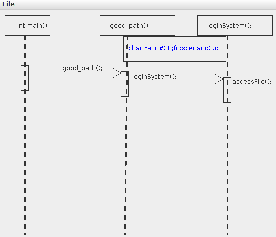
\includegraphics[width=150mm,scale=.50]{styles/errorTracePath.pdf}}
	\label{Error_trace_path}
	\caption{Error trace path in UML sequence diagram}
\end{figure}

The process of creating sequence diagram using Java programming language is given below as an algorithm representation. To develop the sequence diagram a separate class is included inside the smtcodan project. The class name is SequenceDiagramGenerator. Inside this class the drawSequenceDiagram function creates the diagram. The function input parameter is a list of IASTNode which is delivered from the smtcodan project packages. To draw the diagram BufferedImage, Graphics2D, JPanel, JFrame  classes were used. At first need to declare object each of these(BufferedImage, Graphics2D, JPanel, JFrame) classes. Then iterating through the list of IASTNodes set all the statements except function call with line number and file name. There is a class which is responsible to draw the visual things of the sequence diagram named MyCanvasDraw. Afterwards need to create an object of this class. This class has a list. The list of this class has to be set with the list of all statements, line number  and file name. Then it will draw the diagram according to the list. To view this diagram need to set the JFrame object and make it visible. Inside the JFrame JScrollpane object also added to make the frame scrollable. For saving the diagram as an image save as option also included. Through the menu bar user can easily save the sequence diagram as an image. By default it will save the image as in .jpg format. But one can easily save this image in other format like .png,.bmp,.jpeg etc. Exit option is also included inside the JFrame through which user can exit the current window.  


\begin{algorithm}
	{\textbf{Sequence diagram generator}}\\	
	\noindent\makebox[\linewidth]{\rule{\textwidth}{0.4pt}}
	{\textbf{Input: List of statements and function call}} \\
	{\textbf{Output: Sequence diagram in a frame}}
	\begin{algorithmic}[1]
		
		\Function{drawSequenceDiagram}{$ArrayList<IASTNode> statementsList$}
		    \State $ Frame (object)  $ 
			\State $ BufferedImage (object)  $ 
			\State $ Graphics2D(object) $
			\State $ Panel (object)$
			\State $ MyCanvasDraw(object )  $
			\For{$i:statementsList.size()$} 
				\If {$!statementsList.get(i).getRawSignature().toString().contains("(")$}
					
					\State $int j=i;$
					\If{$j<=statementsList.size()-2$}
						\State $do$
						\State $add(ln)$ \Comment{ln=line number}
						\State $add(fn)$ \Comment{fn=file name}
						\State $while(!statementsList.get(j).getRawSignature().toString().contains("("))$
						\State $mcd.buggyPathList.add(allStatements);$ \Comment{Where allStatements - statements of C}
					\EndIf				
				\EndIf		
				
			\EndFor
				\State $set <- ScrollPane(property)$
				\State $mcd.paint(graphics2D)$ \Comment{Where mcd = MyCanvasDraw object}
				\State $topPanel.add(mcd)$ \Comment{Where topPanel = Panel object}	
				\State $menuBar <- MenuBar$
				\State $menuFile <- Menu $
				\State $menuFileExit <- MenuItem$
				\State $menuSaveAs <- MenuItem $
				\State $menuSaveAs.addActionListener <- fileSave and exit$
				\State $set<-frame (properties=visibility,menubar)$
		
		\EndFunction		
		
	\end{algorithmic}
	\noindent\makebox[\linewidth]{\rule{\textwidth}{0.4pt}}
\end{algorithm}

		\chapter{Experiments}
\section{Authentication Scenario:}

In the following Java example the method createDBAccess is used to create a DBAccess object for a database management application.

\begin{lstlisting}
public DBAccess createAccount(String userName, String userType,
 String userPassword) {

		DBAccess access = new DBAccess();
		access.setUserName(userName);
		access.setUserType(userType);
		access.setUserPassword(userPassword);	
				
		return access;
}

\end{lstlisting}

However, there is no authentication mechanism to ensure that the user creating this database user account object has the authority to create new user access. Some authentication mechanisms should be used to verify that the user has the authority to create database access objects.
The following Java code includes a boolean variable and method for authenticating a user. If the user has not been authenticated then the createAccount will not create the database access object.

\begin{lstlisting}

private boolean isUserAuthentic = false;

// authenticate user,
// if user is authenticated then set variable to true
// otherwise set variable to false
public boolean authenticateUser(String username, String password) {
...
}

public DBAccess createAccount(String userName, String userType,
String userPassword) {
			DBAccess access = null;
			
			if (isUserAuthentic) {
			access.setUserName(userName);
			access.setUserType(userType);
			access.setUserPassword(userPassword);
		}
	return access;
}
\end{lstlisting}

Now let's model this kind of scenario in UML statechart considering that for C/C++ application.

\begin{figure}[htbp]
	\centering
	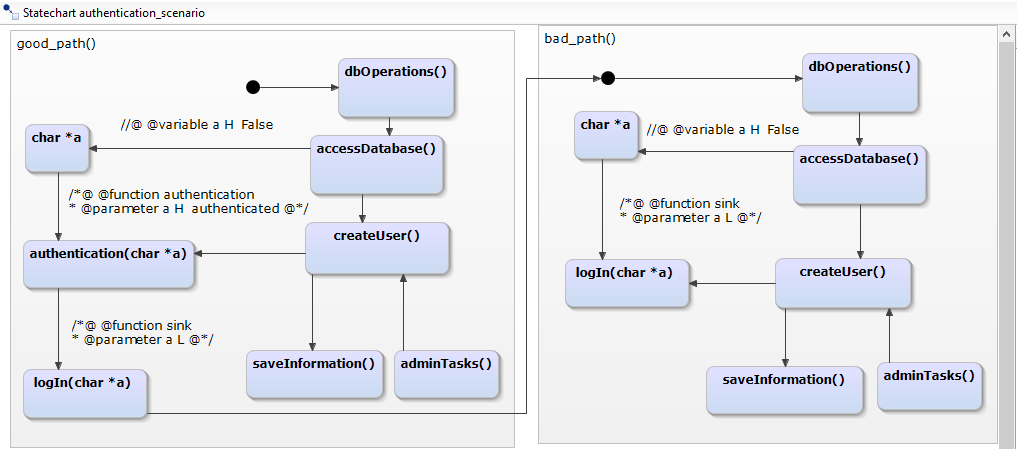
\includegraphics{styles/authentication_scenario.png}
	\caption{Authentication Scenario}
\end{figure}

\section{Declassification Scenario:}
 Noninterference is typically
 too strong a property, most programs use some form of declassification to selectively leak high security information, e.g. when performing a password check or data encryption. Unfortunately, such  a declassification is often expressed as an operation within a given  program, rather than as part of a global policy, making reasoning about the security implications of a policy more difficult. For application programmers need to prevent a range
 of problems, from SQL injection and cross-site scripting, to inadvertent password disclosure and missing access control checks.Adding declassification function is one of the possibility for an application to detect information flow vulnerabilities. It requires few changes to the existing application code and an assertion of functions such as declassification, sanitization and authentication can reuse existing code and data structures. \\
 
 For the declassification scenario, a user A wants to access his bank account. Every bank has their own policy to their customer who can access their account information. After giving the password, account number, user name user A send his request to the bank server to view the account information. The bank server has his own policy according to their requirements. Through that policy bank server verifies the user A may be by following the basic declassification goals according to four axes like what information is released,
 who releases information, where in the system information is released and when information can be released.  \\
 
 Figure \ref{declassification_scenario}  represents a declassification scenario. In this scenario a user A wants to access his bank account. At first he/she has to provide his/her user id, password, account number. Then he/she sends request to access his/her account. The bank server has their own policy who can access the account details. According to the policy user can either view his account details or not. If bank server doesn't have some secured policy like encryption, decryption or declassification methodology then hacker may easily break the application and receives the confidential information or data. In Figure \ref{declassification_scenario} depicts a highly secured variable \enquote{char *a} which is initially annotated as H. It passes through a function named declassification. This declassification function is represented as a state in the statechart as like \enquote{void declassification(char *a)}. This function makes the high secured variable as low by following the policy language. After passing these function the variable \enquote{char *a} is annotated with L and declassified. Now it can be passed to other function or release information to the verified user.\\
 
 After finishing the modeling of declassification scenario then through the C code generator C code files are generated which consist two files(.c and .h file). Inside those files annotations are exist. Then through static analysis engine named \enquote{smtcodan} analyze the code and detect the information flow vulnerabilities if they exist inside the generated files.
 
\begin{figure}[htbp]
	\centering
	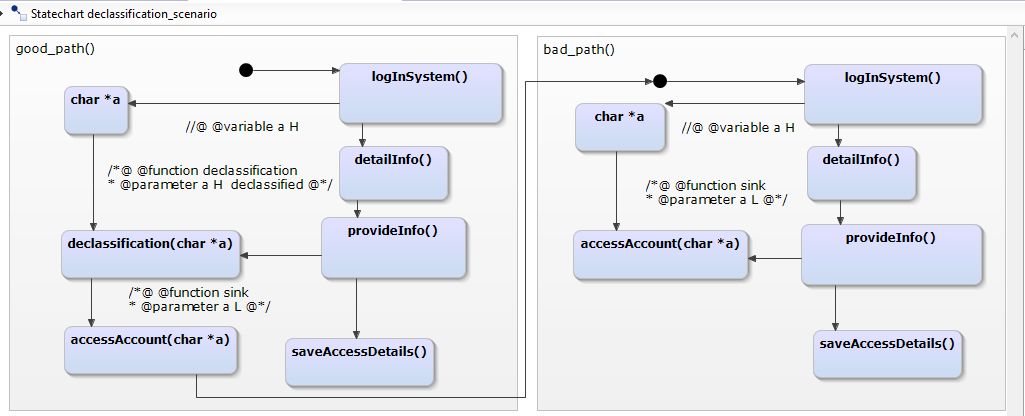
\includegraphics{styles/declassification_scenario.png}
	\label{declassification_scenario}
	\caption{Declassification Scenario}
\end{figure}


\section{Sanitization Scenario:}
Web applications are often implemented by developers with limited security skills.As a result, they
contain vulnerabilities. Most of these vulnerabilities stem
from the lack of input validation. That is, web applications
use malicious input as part of a sensitive operation, without having properly checked or sanitized the input values
prior to their use.
In the past research on vulnerability analysis has mostly focused on identifying cases in which a web application directly uses external input in critical operations. However,
little research has been performed to analyze the correctness of the sanitization process. Secured web application helps to prevent the bad guys from gaining unauthorized access to your application/site's data. It helps you keep your data's integrity and ensures availability as needed. Sql injection and XSS attacks are common attacks now-a-days. to prevent this kind of attacks need to use sanitization methods and validate user input properly.\\
This example code intends to take the name of a user and list the contents of that user's home directory. It is subject to the first variant of OS command injection.Example language is in PHP.

\begin{lstlisting}
	$userName = $_POST["user"];
	$command = 'ls -l /home/' . $userName;
	system($command);
\end{lstlisting} 

The userName variable is not checked for malicious input. An attacker could set the userName variable to an arbitrary OS command such as:
\begin{lstlisting}
;rm -rf /
\end{lstlisting}
Then that would produce a result like this-
\begin{lstlisting}
ls -l /home/;rm -rf /
\end{lstlisting}
Since the semi-colon is a command separator in Unix, the OS would first execute the ls command, then the rm command, deleting the entire file system.\\

The previous example was given for PHP language. In C language here it has been selected that user \enquote{A} wants to access some file from server pc. So, he needs to give the file name. If he wants to access some exe file then bug should be triggered or if he inserts some OS command injection type of statement then bug should be triggered. That's why the user input should pass through a sanitization method to sanitize the input parameter.\\

 Figure \ref{sanitization_scenario} depicts a sanitization scenario. In this scenario a user A wants to access file from a server. At first he/she has to provide file name. Then he/she sends request to access his/her desire file. The server has their policy who can access the file. According to the policy if the server has proper sanitization methods then by sanitizing the user input server either allow or disallow the user to access the file. If bank server doesn't have some secured policy like encryption, decryption or sanitization methodology then hacker may easily break the application and receives the confidential information or data, even execute the .exe files or may do some OS command injection. In Figure \ref{sanitization_scenario} shows a highly secured variable \enquote{char *a} which is initially annotated as H. It passes through a function named sanitization which also represented as a state named \enquote{void sanitization(char *a)}. This function makes the high secured variable as low by following the policy language. After passing these function the variable \enquote{char *a} is annotated with L and sanitized. Now it can be passed to other function or release information from the system.

\begin{figure}[htbp]
	\centering
	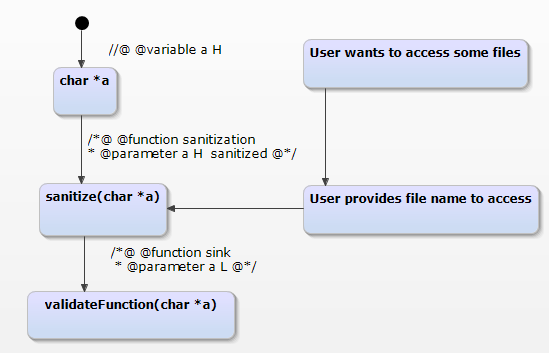
\includegraphics{styles/sanitization_scenario.png}
	\label{sanitization_scenario}
	\caption{Sanitization Scenario}
\end{figure}
		\chapter{Related Work}

There are many annotation languages proposed until now for
extending the C type system \cite{ref_54_condit:dependent}, \cite{ref_53_evans:static,ref_51_microsoft:sal,ref_55_sun:lock,ref_56_torvalds:sparse} to be
used during run-time as a new language run-time for PHP and
Python \cite{ref_57_alex:improving} to annotate function interfaces \cite{ref_53_evans:static,ref_51_microsoft:sal,ref_56_torvalds:sparse} to
annotate models in order to detect information flow bugs \cite{ref_27_iflow:kuzman}
to annotate source code files \cite{ref_59_rosenblum:towards,ref_60_rosenblum:practical,ref_61_lintan:acomment} or to annotate
control flows \cite{ref_53_evans:static,ref_52_splint:flow,ref_51_microsoft:sal}. The following annotation languages have made significant impact: Microsoft\'s SAL annotations \cite{ref_51_microsoft:sal} helped to detect more than 1000 potential security vulnerabilities in Windows
code \cite{ref_50_ball:research}. In addition, several other annotation languages including  Jif \cite{ref_48_chong:jif}, AURA \cite{ref_46_jia:aura}, FlowCaml \cite{ref_32_simonet:report}, FINE \cite{ref_45_nikhil:fine} and Fable \cite{ref_47_swamy:fable} express information flow related concerns.

Saner \cite{ref_61_lintan:acomment}, a novel approach to the evaluation of the sanitization process in web applications. The approach relies on two complementary analysis techniques to identify faulty sanitization procedures. Saner \cite{ref_61_lintan:acomment} introduce a dynamic analysis technique that is
able to reconstruct the code that is responsible for
the sanitization of application inputs, and then execute this code on malicious inputs to identify faulty
sanitization procedures. By applying
it to real-world applications, identified novel vulnerabilities that stem from incorrect or incomplete sanitization.

A simple idea named trusted declassification \cite{ref_2_hicks2006trusted} in which special declassifier functions are specified as part of the global policy. In particular, individual principals declaratively specify which declassifiers they trust so that all information flows implied by the policy can be reasoned about in absence of a particular program. They formalize their approach for a Java like language and prove a modified form of noninterference which they call noninterference modulo trusted methods. They have implemented their approach as an extension to Jif and provide some of their experience using it to build a secure e-mail client.

Using RESIN \cite{ref_63_yip2009improving}, Web application programmers can prevent a range
of problems, from SQL injection and cross-site scripting, to inadvertent password disclosure and missing access control checks. Adding
a RESIN assertion to an application requires few changes to the
existing application code, and an assertion can reuse existing code
and data structures. For instance, 23 lines of code detect and prevent
three previously-unknown missing access control vulnerabilities in
phpBB, a popular Web forum application. Other assertions comprising tens of lines of code prevent a range of vulnerabilities in Python
and PHP applications. A prototype of RESIN incurs a 33\% CPU
overhead running the HotCRP conference management application.

Static code analysis is a way to find bugs and reduce the defects in a software application. In the 1970's, Stephan Johnson at Bell Laboratories, wrote Lint, a tool to examine C
source programs that had compiled without errors and to find bugs that had escaped detection. There are many ways to detect and reduce the number of bugs in a program. In Java, JUnit is a very useful tool for writing tests. Overtime research proved that analyzing the code (especially code reviews) is the best way to eliminate bugs. This is not
always possible because it is very hard to train people and get them together to study and identify problems in programs. Furthermore it is almost impossible to use code inspections on project's complete code base.
Most errors fall into known categories, as people tend to fall into the same traps repeatedly. Therefore a static analyzer or checker is a program written to analyze other programs for flaws. 

UMLSec \cite{ref_33_juerjens:secure} is a model-driven approach that allows the
development of secure applications with UML. Compared with
our approach, UMLSec does neither automatic code
generation nor the annotations can be used for automated
constraints checking.

TAJ \cite{ref_100_tripp2009taj}, an approach to taint analysis suitable for industrial applications. An experimental evaluation indicates that
the hybrid algorithm TAJ uses for slice construction is an attractive
compromise between context-sensitive and context-insensitive
thin slicing. TAJ is able to perform effective taint analysis in a limited budget, improving performance without significantly degrading accuracy.

Darvas et al. \cite{ref_70_darvas2005theorem} used a self-compositional approach to prove secure information flow properties for Java CARD programs. They used an interactive approach instead of an automatic approach. Barthe et al. coined the term "self-composition" in their paper \cite{ref_71_barthe2004secure}. Their paper is mostly theoretical results on characterizing various secure information flow problems, including
non-deterministic and termination-sensitive cases, in a self-compositional framework.

Wassermann et al. \cite{ref_102_minamide2005static} string-analysis algorithm to syntactically isolate tainted substrings from untainted
substrings in PHP applications. They labeled non-terminals in a
Context-Free Grammar (CFG) with annotations reflecting taintedness
and untaintedness. Their expensive, yet elegant mechanism
is applied to detect both SQL injection and XSS vulnerabilities.

McCamant et al. \cite{ref_101_mccamant2008quantitative} take a quantitative approach in information
flow: instead of using taint analysis, they cast information-
flow security to a network-flow-capacity problem, and describe a
dynamic technique for measuring the amount of secret data that
leaks to public observers.

Barthe et al. \cite{ref_71_barthe2004secure} showed that their self compositional framework can handle delimited information release as originally proposed by Sabelfeld et al. \cite{ref_72_sabelfeld2004model}. Li et al.
recently proposed relaxed non-interference \cite{ref_73_li2005downgrading} is equivalent to delimited information release when strengthened with semantic equivalence. Relaxed non-interference is arguably a more natural formulation of information downgrading than delimited
information release. This research suggests a promising practical approach of natural formulation of information downgrading.


The detection of information flow errors can be
addressed with dynamic analysis techniques \cite{ref_44_avgerinos:aeg,ref_43_fenton:memoryless,ref_42_sabelfeld:dynamic},
static analysis techniques \cite{ref_41_guarnieri:security,ref_40_myers:jflow,ref_38_volpano:sound,ref_37_xiao:transparent} (similar
to our approach with respect to static analysis of code and
tracking of data information flow) and hybrid techniques which
combine static and dynamic approaches \cite{ref_36_moore:static}. Also, extended
static checking \cite{ref_35_david:extended} (ESC) is a promising research area which
tries to cope with the shortage of not having certain program
run-time information.
The static code analysis techniques need to know which
parts of the code are: sinks, sources and which variables
should be tagged. A solution for tagging these elements in
source code is based on a pre-annotated library which contains
all the needed annotations attached to function declarations.
Leino \cite{ref_34_leino:10years} reports about the annotation burden as being very
time consuming and disliked by some programming teams.

Security concerns are a major disincentive for use of the
cloud, particularly for companies responsible for sensitive
data. DIFC \cite{ref_74_bacon2014information} is most appropriately integrated into a PaaS cloud model which can be tested by augmenting
existing open source implementations such as VMware CloudFoundry
and Red Hat OpenShift. DIFC has been used to protect user
data integrity and secrecy. In order to apply these techniques
to a cloud environment a number of challenges need to be
overcome. These include: selecting the most appropriate DIFC
model; policy specification, translation, and enforcement; audit
logging to demonstrate compliance with legislation and for
digital forensics.

There exist several approaches that are focused on the detection of "taint-style" vulnerabilities (such as XSS or SQL injections), which
frequently occur in web applications. Huang et al. \cite{ref_75_huang2004securing}
adapted parts of the techniques used in CQual to develop
an intraprocedural analysis for PHP programs. In \cite{ref_76_huang2004verifying}, the
same authors presented an alternative approach that is based
on bounded model checking. Whaley et al. \cite{ref_77_whaley2004cloning} described an interprocedural, flow-insensitive alias analysis for Java applications. Their analysis is based on binary decision diagrams and was used by Livshits et al. \cite{ref_78_livshits2005finding} for the detection of taint-style vulnerabilities. In \cite{ref_62_balzarotti2008saner}, their approach is based on Pixy \cite{ref_80_jovanovic2006precise,ref_79_jovanovic2010static}, an open
source static PHP analyzer that uses taint analysis for detecting XSS vulnerabilities.

Weinberger et al. empirically studied present sanitization
approaches against XSS in web application frameworks \cite{ref_105_weinberger2011systematic}.
They analyzed the availability of sanitization approaches for
different HTML markup contexts for five PHP frameworks.
Furthermore, eight PHP applications were studied for the
usage of various markup contexts. A templating framework
was proposed by Samuel et al. that uses type qualifiers
to automate context-sensitive XSS sanitization \cite{ref_106_samuel2011context}.

A good overview of static analysis approaches applied to security problems are provided in \cite{ref_18_chess2004static}. Simple lexical approaches employed by scanning tools such as ITS4 and RATS use a set of predefined patterns to identify potentially dangerous areas of a program \cite{ref_82_wilander2002comparison}. While a significant improvement on Unix grep, these tools, however, have no knowledge of how data propagates throughout the program and cannot be used to automatically and fully solve taint-style problems.
A few projects use path-sensitive analysis to find errors in C and C++ programs \cite{ref_83_bush2000static,ref_84_hallem2002system,ref_85_livshits2003tracking}. While capable of addressing taint-style problems, these tools rely on an unsound approach to pointers and may therefore miss some errors. The WebSSARI project uses combined unsound static and dynamic analysis in the context of analyzing PHP programs \cite{ref_75_huang2004securing}. WebSSARI has successfully been applied to find many SQL injection and cross-site scripting vulnerabilities in PHP code.

 The studies rely on manually
written annotations while our annotation language is integrated
into two editors which are used to annotate UML state
charts and C code by selecting annotations from a list and
without the need to memorize a new annotation language.

Recently taint modes integrated in programming languages as Camlbased FlowCaml \cite{ref_32_simonet:report}, Ada-based SPARK Examiner \cite{ref_31_chapman:enforcing} and the scripting. However, none of these annotation and programming languages have support for introducing information flow
restrictions in both models and the source code.
Splint \cite{ref_30_david:splint}, Flawfinder \cite{ref_29_wheeler:flawfinder} and Cqual \cite{ref_28_umesh:cqual} are used to detect information flow bugs in source code and come with
comprehensive user manuals describing how the annotation
language can be used in order to annotate source code.
iFlow \cite{ref_27_iflow:kuzman} is used for detecting information flow bugs in
models and is based on modeling dynamic behavior of the
application using UML sequence diagrams and translating
them into code by analyzing it with JOANA \cite{ref_26_kit:joana}. In comparison with our approach these tools do not use the same
annotation language for annotating UML models and code.
Thus, a user has to learn to use two annotation languages
which can be perceived to be a high burden in some scenarios.


 Heldal et al. \cite{ref_25_heldal:bridging,ref_23_heldal:supporting} introduced an
UML profile that incorporates a decentralized label model into the UML. It allows the annotation of UML artifacts with
Jif \cite{ref_48_chong:jif} labels in order to generate Jif code from the UML
model automatically. However, the Jif-style annotation already
proved to be non-trivial on the code level \cite{ref_22_preibusch2011information}, while \cite{ref_23_heldal:supporting}
notes that the actual automatic Jif code generation is still a future
work. These approaches can not be used to annotate both UML
models and code. Moreover, these approaches lack of tools for
automated checking of previously imposed constraints.
		\chapter{Conclusion and Future Works}

In the conclusion and future work we will discuss about the possible future works of this research and conclusion.

\section{Conclusion}
A keyword-based annotation language that can be used out of the box for annotating UML state charts and C code in two software development phases by providing two editors for inserting security annotations in order to detect information flow bugs automatically. It is evaluated on some sample programs and showed that this approach is applicable to real life scenarios.

Functions are used to declassify sensitive data because they are trusted to release information. Our work introduces a security-typed language. We annotate functions with security levels. Functions may be annotated with a high security level; this indicates they are trusted and permits them to serve as a safe mechanism for declassification.

Web applications perform a lot of critical tasks and
handle sensitive information. Even though there have been
a number of research efforts to identify the use of unvalidated input in web applications, little has been done
to characterize how sanitization is actually performed and
how effective it is in blocking web-based attacks. In case of desktop applications it is not easy to handle sensitive information. To handle these sensitive information and invalidate insecure input data a good approach to the evaluation of the sanitization process has been developed. Future work will focus on the analysis of type-based validation procedures.

Mechanisms such as access control, encryption, firewalls, digital
signatures and antivirus scanning do not address the fundamental
problem: tracking the flow of information in computing
systems. Run-time monitoring of operating-systems calls is
similarly of limited use because information-flow policies are
not properties of a single execution; in general, they require
monitoring all possible execution paths. On the other hand,
there is clear evidence of benefits provided by language-based
security mechanisms that build on technology for static analysis
and language semantics. Type systems are attractive for
implementing static security analyses. It is natural to augment
type annotations with security labels. Type systems allow for
compositional reasoning, which is a necessity for scalability
when applied to larger programs. Semantics-based models
are suitable for describing end-to-end policies such as
noninterference and its extensions. These models allow for a
precise formulation of the attacker's view of the system. This
view is described as a relation on program behaviors where
two behaviors are related if they are not distinguishable by
the attacker. Attackers of varying capabilities can be modeled
straightforwardly as different attacker views, and correspond
to different security properties. A number of further advantages are
associated with both security-type systems and semantics based
security. Compositionality is especially valuable in the
context of security properties.Compositionality
greatly facilitates correctness proofs for program analyses. If the recent
progress in language-based techniques for soundly enforcing
end-to-end confidentiality policies continues, the approach
may soon become an important part of standard security
practice.

Last but not least, it is a system which is usable for specifying information flow security constraints which can be used in the design and coding phase in order to detect information flow bugs.





\section{ Future Works}
In future it can be extended for source code editor as
a pop-up window based proposal editor used to add/retrieve
annotation to/from a library. The definition of new language
annotation tags should be possible from the same window by
providing two running modes (language extension mode and
annotation mode). The envisaged result is to reduce the gap
between annotations insertion/retrieval and the definition of
new language tags. This would help to create personalized
annotated libraries which can be collaboratively annotated if
needed.

Currently code generator, UML statechart modeling developed only for windows operating system. In future code generator, state chart editor should be implemented for other operating systems. Another avenue of future work lies in expanding the policy
language. It is currently very simple, but could be more expressive. For example, constraints could be added to indicate negative information flows. Policy analyses could also be used to determine whether separation of duties is maintained between two principals. When integrity is added to policy language, it could be expanded with robustness constraints. It is a general problem in language based security that there is too little experience with security-typed programming to help guide such research as designing the best form of declassification. We hope that our implementation of this mechanism will help to promote more practical experience with declassifiers which will be implemented in future research.



		
		% ---------------------------------------------------------------------------
		%
		% Appendix
		%
		% ---------------------------------------------------------------------------
		
		\part*{Appendix}
		\addcontentsline{toc}{part}{Appendix}
		
		\appendix %---------------------------------------
		
		\chapter{Appendix}
\section{Appendix A: Source Code Editor with Annotation Language}
\lstinputlisting[numbers=left,firstnumber=1,firstline=1]{sourceCode/MyDsl.xtext}

\section{Appendix B: C Code Generator}	

	\lstinputlisting[numbers=left,firstnumber=1,firstline=1]{sourceCode/Naming.xtend}
	
	\lstinputlisting[numbers=left,firstnumber=1,firstline=1]{sourceCode/Types.xtend}
	
\section{Appendix C: Three Checkers in Static Analysis Engine}

\section{Appendix D: Sequence Diagram Generator}

		
	


  \clearemptydoublepage
  
	\bibliography{bibliography/literature}
	
 
\end{document}

